\documentclass[12pt]{article}
\usepackage{amsmath,amssymb,amsfonts}
\usepackage{algorithmic}
\usepackage{booktabs}
\usepackage{graphicx}
\let\PrismOriginalIncludegraphics\includegraphics
\renewcommand{\includegraphics}[2][]{%
    \IfFileExists{#2}{%
        \PrismOriginalIncludegraphics[#1]{#2}%
    }{%
        \fbox{\parbox{0.9\linewidth}{\centering Missing image: \texttt{\detokenize{#2}}}}%
    }%
}
\usepackage{textcomp}
\usepackage{xcolor}
\usepackage{placeins}
\usepackage{needspace}
\usepackage{dblfloatfix}
\usepackage{titlesec}
\usepackage[margin=1in]{geometry}

% Added hyperref for \autoref functionality
\usepackage[colorlinks=true, linkcolor=black, citecolor=black, urlcolor=black]{hyperref}

% Redefine autoref names to match IEEE style (e.g., "Fig." instead of "Figure")
\def\sectionautorefname{Section}
\def\subsectionautorefname{Subsection}
\def\figureautorefname{Fig.}
\def\tableautorefname{Table}

\titleformat{\section}{\bfseries}{\thesection}{1em}{}
\titleformat{\subsection}{\bfseries}{\thesubsection}{1em}{}
\titleformat{\subsubsection}{\bfseries}{\thesubsubsection}{1em}{}
\titleformat{\paragraph}{\bfseries}{\theparagraph}{1em}{}
\title{\large MPC-Net: \underline{M}inkowaski-Distance, \underline{P}arseval-Inequality influenced \underline{C}hoquet-Integral fusion of Gabor-CNN and Swin-CNN for Blood Cell Classification}

\author{%
Debatra Banerjee\\[0.5em]
\normalsize Under supervision of Mahantapas Kundu\\[0.25em]
\normalsize Class: BCSE UG-4, Section: A2, Roll: 002210501099\\[0.25em]
\normalsize Department of Computer Science and Engineering, Jadavpur University, Kolkata, India\\[0.25em]
}
\date{}

\begin{document}

\maketitle


\begin{abstract}
In this paper,we propose MPC-net a novel lightweight dual-branch deep learning architecture for automated blood cell classification that integrates local and global feature representations. The local branch uses a Gabor filter-based CNN to capture fine-grained texture and orientation details, while the global branch employs Shifted Window Multi-head Self-Attention to model long-range dependencies. A Choquet integral-inspired fuzzy fusion mechanism, enhanced with Minkowski distance and Parseval-based energy alignment, adaptively combines these complementary features for improved robustness and discrimination. The proposed method achieves 97.07\% accuracy on BloodMNIST and 95.31\% on the Raabin-WBC dataset, outperforming several state-of-the-art approaches.%The results highlight the potential of hybrid architectures with advanced fusion strategies for medical image classification tasks
\end{abstract}

\noindent\textbf{Keywords:} Blood Cell Classification; CNN; Gabor Filters; Swin Attention; Choquet Integral; Minkowski Distance; Parseval Inequality; Early Fusion

\section{Introduction}

Hematological disorders, including leukemia, remain a major global health concern due to their rapid progression and high mortality when not detected early. Accurate classification of blood cell types is a critical step in diagnosis, as subtle morphological differences in white blood cells often indicate underlying pathological conditions. With early advancements in Computer Vision–based Computer-Aided Diagnosis (CAD) systems, automated approaches have been developed to assist clinicians by improving efficiency, consistency, and scalability compared to traditional manual microscopy.

Despite these advancements, blood cell classification remains inherently challenging. Blood cells exhibit significant intra-class variability while often sharing strong visual similarities across classes, making discrimination difficult even for experienced experts. Factors such as staining inconsistencies, illumination variations, and overlapping cells further degrade image quality and complicate feature extraction.

In addition, diagnostically relevant information exists at multiple spatial scales. Fine-grained details like chromatin texture and cytoplasmic granularity must be interpreted alongside higher-level structural features such as nucleus shape and cell boundaries. Effectively capturing and integrating these diverse characteristics within a single model continues to be a central challenge, motivating the development of more robust and adaptive deep learning-based classification frameworks.


Conventional convolutional neural networks (CNNs) (Alzubaidi Laith et al.~\cite{b37}) have demonstrated strong performance in medical image classification due to their ability to learn hierarchical feature representations. However, standard CNNs are inherently biased toward local receptive fields and may fail to effectively capture long-range dependencies and global contextual information. On the other hand, attention-based models such as transformers can model global relationships but often lack sensitivity to fine-grained texture details and may introduce additional computational complexity. As a result, relying solely on either local or global feature modeling is insufficient for robust blood cell classification.

Motivated by these challenges, this work explores a hybrid dual-branch architecture that explicitly models both local and global feature representations and integrates them through a principled fusion mechanism. The local branch leverages \textbf{Gabor filter}-based convolutional operations as shown by Mehrotra et al.~\cite{b33}, to capture orientation-sensitive micro-textural patterns, which are critical for distinguishing subtle cellular structures. In parallel, the global branch incorporates \textbf{Shifted Window Attention} as given by Liu, Ze et al.~\cite{b34} to efficiently model long-range dependencies and contextual relationships across the image. A key contribution of this work lies in the proposed fusion strategy. Instead of conventional fusion techniques such as concatenation or averaging, we introduce a \textbf{Choquet integral}-inspired fuzzy aggregation framework, given by Grabisch et al.~\cite{b35} that accounts for interaction between feature sources. This formulation is further enhanced using \textbf{Minkowski distance}, as found in Xu, Hang et al.~\cite{b36} to model geometric divergence and \textbf{Parseval theorem}-based energy alignment to capture semantic agreement. Together, these components enable adaptive, interaction-aware fusion that reinforces complementary information while suppressing conflicting evidence.

The proposed approach is evaluated on benchmark datasets including BloodMNIST and Raabin-WBC, demonstrating strong performance and improved generalization. Through both quantitative results and qualitative analyzes, we show that effective integration of local and global representations, combined with principled fusion, leads to improved discriminative capability and interpretability in blood cell classification tasks.
\subsection{Contributions}

The main contributions of our work are summarized as follows:

\begin{enumerate}

\item \textbf{Dual-branch architecture for complementary feature learning:}  
We propose MPC-net a lightweight unified dual-branch framework that explicitly models both local and global representations from blood cell images. The local branch leverages Gabor-filter-based convolutions to capture fine-grained texture and orientation patterns, while the global branch integrates shifted window attention to efficiently encode long-range spatial dependencies. This design enables the model to capture many multi-scale morphological characteristics.

\item \textbf{Interaction-aware fuzzy fusion mechanism:}  
We introduce a novel Choquet integral-inspired fusion strategy that models non-linear interactions between feature sources. Unlike conventional fusion methods such as concatenation or averaging, the proposed formulation employs an adaptive fuzzy measure $\mu$ that adjusts dynamically, allowing super-additive aggregation when features agree and sub-additive behavior when they diverge.

\item \textbf{Geometric and energy-aware feature integration:}  
To enhance the classical Choquet formulation, we incorporate Minkowski distance-based modulation to account for geometric divergence between feature embeddings, and Parseval-based energy alignment to capture semantic agreement. This combined mechanism enables robust suppression of conflicting information.

\item \textbf{Comprehensive evaluation and interpretability analysis:}  
The proposed model is extensively evaluated on benchmark datasets including BloodMNIST and Raabin-WBC, achieving strong performance compared to state-of-the-art methods. Ablation studies validate the contribution of each component, while Grad-CAM and t-SNE analyses provide qualitative evidence of our superior fusion model.

\end{enumerate}

\subsection{Literature Survey}

Automated blood cell classification has attracted significant attention in medical image analysis due to its importance in diagnosing hematologic disorders. With the advancement of deep learning, CNNs have become widely used for microscopic blood cell image classification. Posada et al. (2022) ~\cite{b43} proposed meta-learning paradigm with XceptionNet prior-model at the meta-level and with Support Vector Machine (SVM) at the base level and achieved 94.4\% accuracy on the Raabin-WBC dataset. Shobiry et al. (2025) \cite{b17} investigated whether EfficientNetV2 or ResNet50 features yield better separability for BloodMNIST. They tried different classical classifiers such as SVM, Artificial Neural Network (ANN), K-Nearest Neighbors (KNN), and Random Forest. They found that the best trade-off between accuracy, computation time, and model size was given by EfficientNetV2 + SVM with 77\% test accuracy on the BloodMNIST dataset.

In ensemble based approaches, Dhibar et al. (2025) ~\cite{b41} proposed a technique consisting of an ensemble of three CNN networks for Raabin-WBC classification (DCENWCNet), which achieved  93.93\% accuracy. In Fuzzy based approaches, Zhao et al. (2026)~\cite{b38} proposed a Fuzzy Attention Network Layer (FANL) that integrates intuitionistic fuzzy set theory into attention by modeling feature importance using membership, non-membership, and hesitation degrees to capture uncertainty and achieved 96.25\% test accuracy on the BloodMNIST dataset. O Bilai et al. (2025) ~\cite{b45} proposed a weighted ensemble framework by integrating three advanced pre-trained convolutional neural networks (CNNs): DenseNet169, DenseNet201, and Xception models and acheived 95.23\% in BloodMNIST dataset. Manzari et al. ~\cite{b46} proposed MedViT which combines combines CNNs’ localized feature extraction capabilitieswith the global feature representation of ViTs and acheived 95\% test accuracy on BloodMNIST dataset. Sengupta et al. (2025)~\cite{b39} proposed  a graph-based learning framework named FireGNN that integrates trainable fuzzy rules into GNNs for medical image classification and achieved 88.31±0.37\% accuracy using GCN + FR (Fuzzy Rules) on the BloodMNIST dataset.

In Quantum circuit based approach, Radhi et al. (2024)~\cite{b16} proposed a hybrid quantum–classical architecture that combines variational quantum circuits with EfficientNet-based feature extraction for medical image classification and achieved test accuracy of 96.58\% on the BloodMNIST dataset.

In segmentation based approach, Tavakoli et al. (2021) \cite{b42} proposed segmenting the WBC nucleus, generating its convex hull, and deriving a ROC image, which along with RGB and nucleus images is used it to train a custom CNN. Their model achieved an accuracy of 93.97\% on the Raabin-WBC dataset. Tavakoli et al. (2021) \cite{b44} proposed a three-stage method involving nucleus and partial cytoplasm detection (within the nucleus’s convex hull), feature extraction (shape and novel color features), and SVM-based classification. Their model achieved an accuracy of 94.65\% on the RaabinWBC dataset.

Although CNN-based approaches have demonstrated strong performance, they often struggle to capture global contextual relationships due to their localized receptive fields. Consequently, effectively integrating both local structural details and long-range contextual dependencies remains a critical challenge in medical image classification. Motivated by these observations, our work explores a hybrid architecture that leverages complementary feature representations to improve classification performance on microscopic blood cell datasets.


\section{Methodology}

\subsection{Proposed Architecture}

Our proposed lightweight model MPC-net consists of two parallel branches operating on the same input feature map: 
(i) a Gabor-CNN branch for local feature extraction, and 
(ii) a CNN with shifted window attention branch for global dependency modeling. The network contains only $\sim$0.5M parameters, making it substantially more lightweight than standard pretrained architectures.
The outputs of both branches are projected into a shared latent space and fused using a Choquet-inspired fuzzy aggregation enhanced with Minkowski distance and Parseval-based alignment. 
The complete architecture is shown in \autoref{fig:model}.

\begin{figure*}[!b]
    \centering
    \IfFileExists{Untitled Diagram2.jpg}{%
        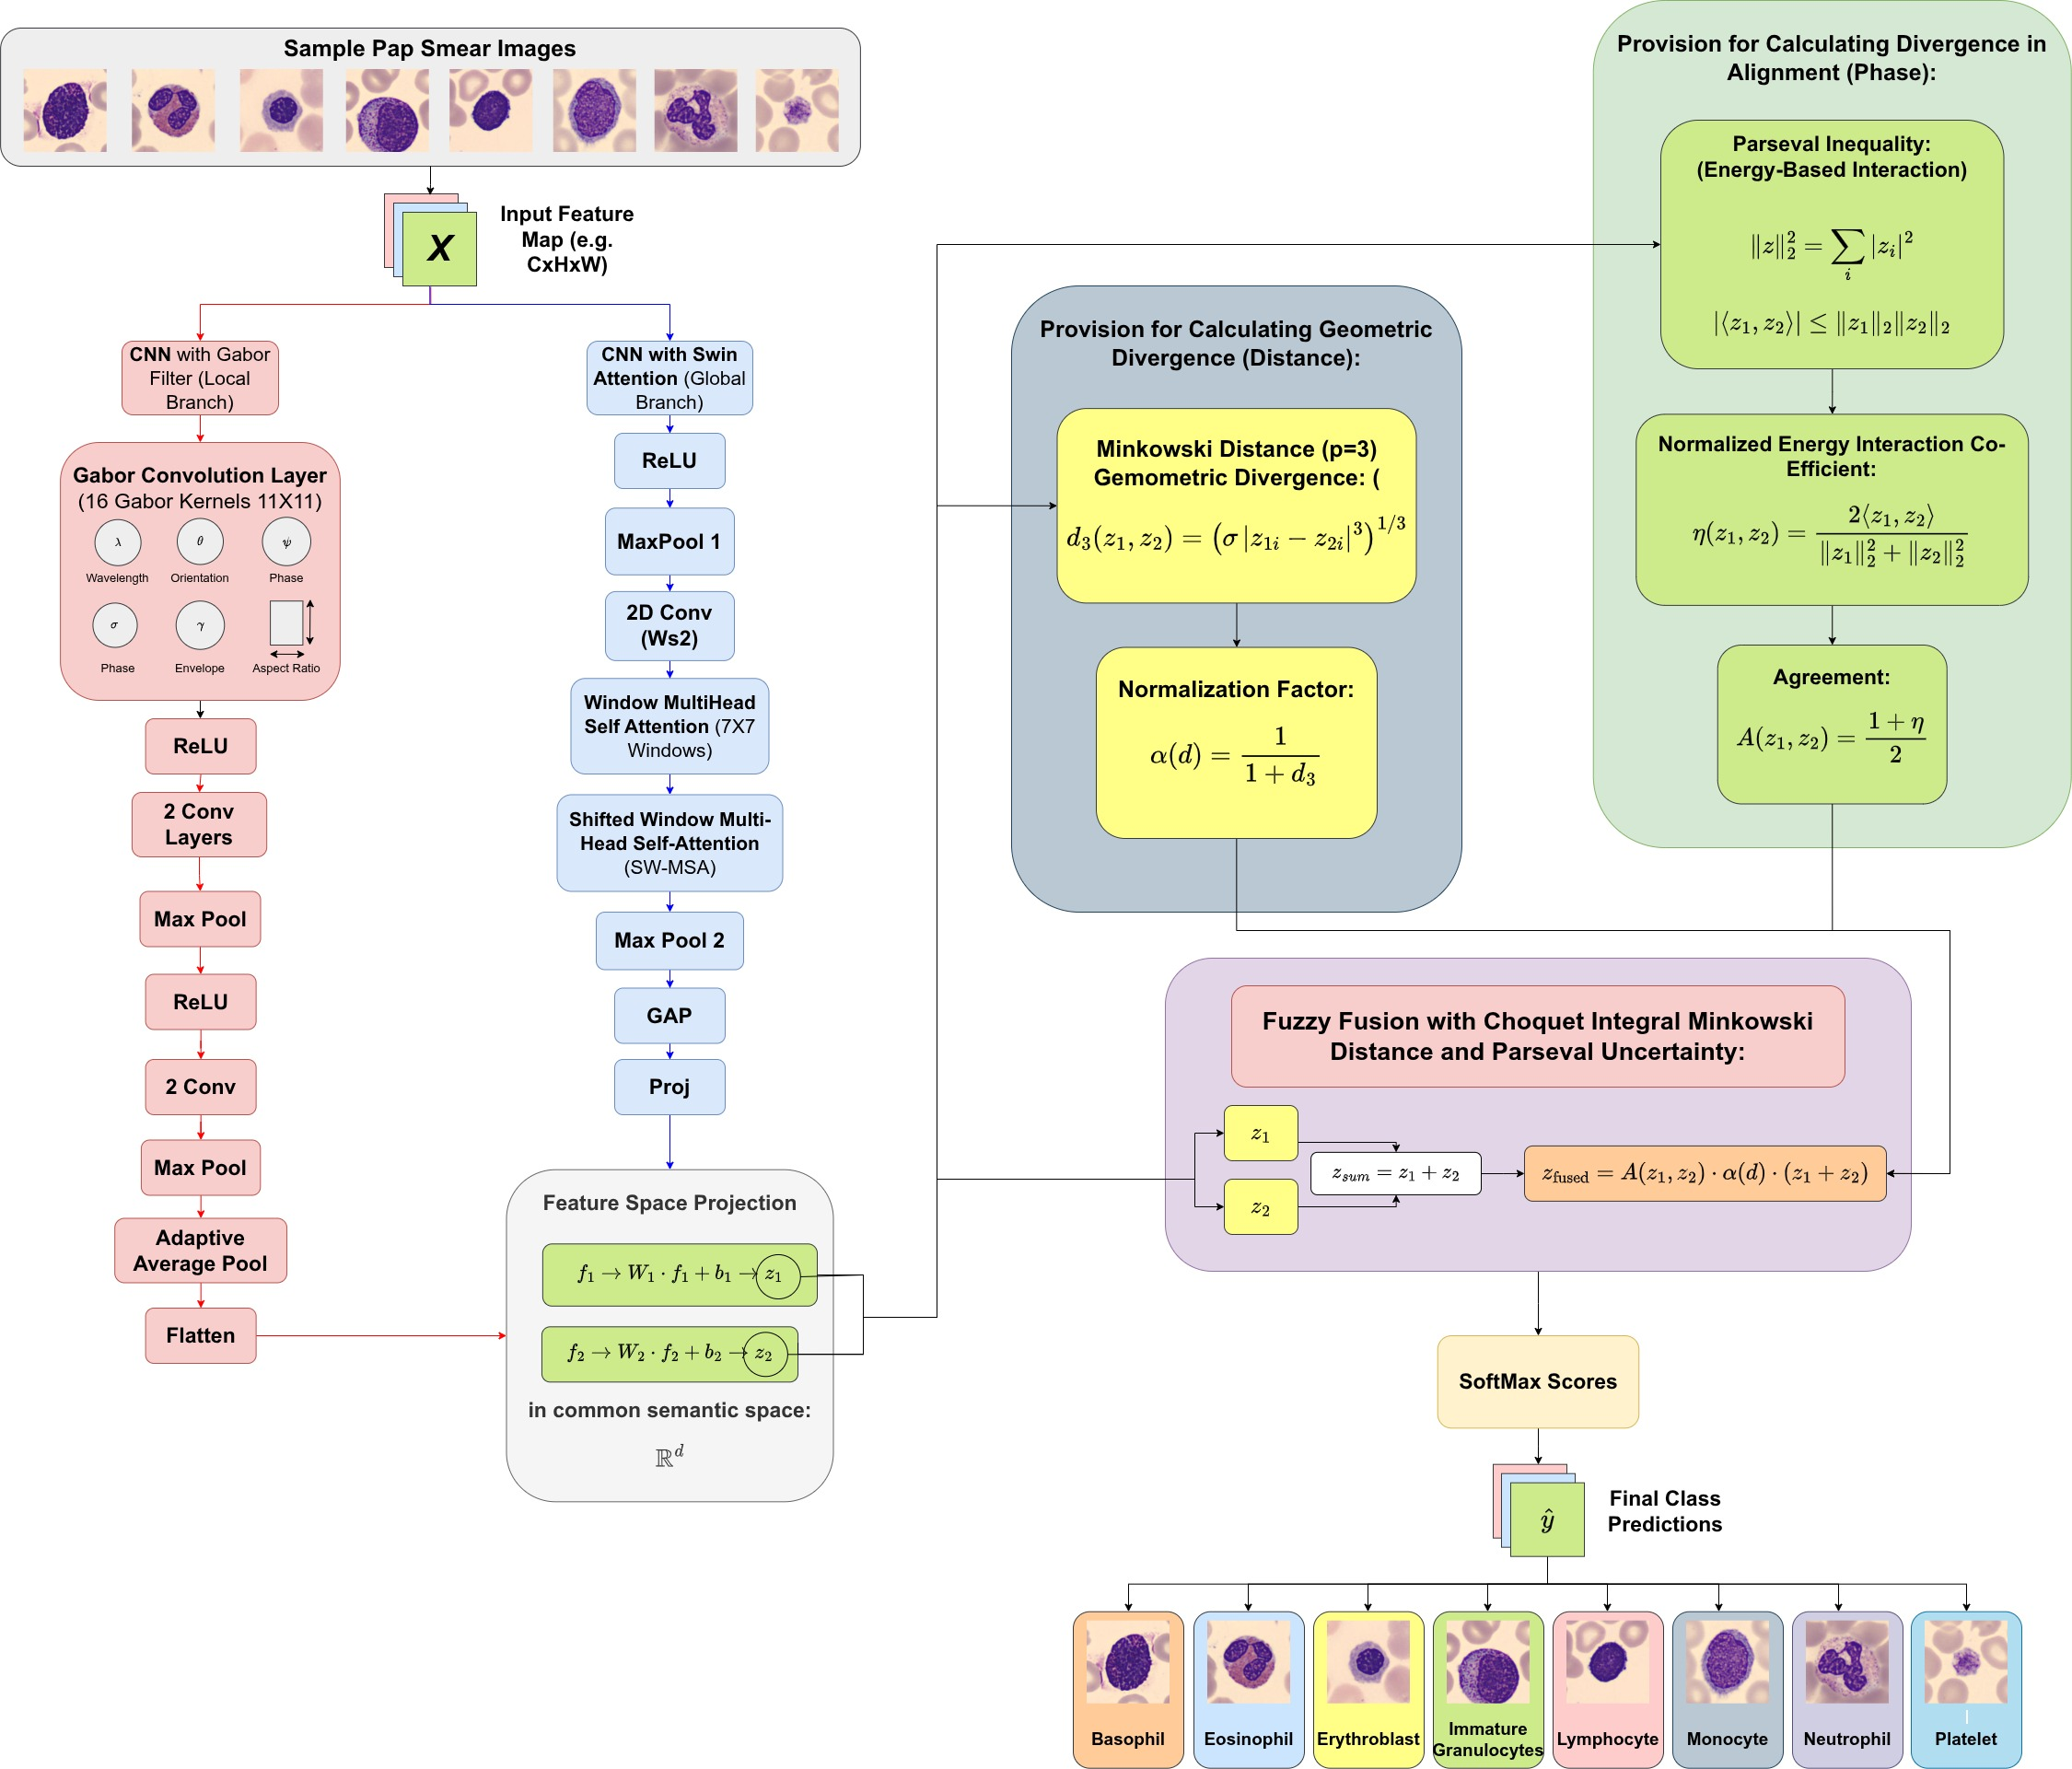
\includegraphics[width=\linewidth]{Untitled Diagram2.jpg}%
    }{%
        \fbox{\parbox{0.9\linewidth}{\centering Architecture figure placeholder: \texttt{Untitled Diagram2.jpg} not found.}}%
    }
    \caption{Architecture of our proposed model. }
    \label{fig:model}
\end{figure*}

\subsection{Feature Extraction}

\subsubsection{Local Branch: Gabor Filter-aided CNN}

The local branch captures fine-grained texture and orientation information using a Gabor convolution layer followed by standard CNN operations. The 2D Gabor kernel ~\cite{b1} is defined as:

\begin{equation*}
g(x, y; \lambda, \theta, \psi, \sigma, \gamma)
=
\exp\left(-\frac{x'^2 + \gamma^2 y'^2}{2\sigma^2}\right)
\cdot
\exp\left(i\left(2\pi \frac{x'}{\lambda} + \psi\right)\right)
\end{equation*}

with rotated coordinates:
\begin{equation*}
x' = x\cos\theta + y\sin\theta,\quad
y' = -x\sin\theta + y\cos\theta
\end{equation*}

Multiple Gabor kernels provide dense orientation coverage, enabling robust detection of edges and textures across directions ~\cite{b2}. This makes the branch particularly effective for capturing micro-structural patterns in blood cell images. The feature extraction pipeline is:

\begin{equation*}
\resizebox{\columnwidth}{!}{$
\mathbf{f}_{local}
=
\mathrm{GAP}\big(
\mathrm{Pool}_2(
\mathrm{ReLU}(
\mathbf{W}_2 *
\mathrm{Pool}_1(
\mathrm{ReLU}(
\mathbf{W}_1 *
\mathrm{ReLU}(
\mathbf{W}_{gabor} * \mathbf{X}
)
)
)
)
)
\big)
$}
\end{equation*}

This hierarchical processing mimics progressively higher-level visual representations, analogous to biological vision systems ~\cite{b3}.


\subsubsection{Global Branch: CNN with Shifted Window Attention}

While the local branch captures fine spatial details, it lacks the ability to model long-range contextual dependencies. To address this limitation, we incorporate shifted window multi-head self-attention, which enables efficient global feature aggregation without incurring full self-attention complexity.

The attention operation ~\cite{b4} is defined as:

\begin{equation*}
\text{Attention}(Q,K,V)
=
\text{Softmax}\left(\frac{QK^T}{\sqrt{d}} + B\right)V
\end{equation*}

where $Q$, $K$, and $V$ denote query, key, and value representations, respectively, and $B$ encodes relative positional bias.

In standard window-based attention, computation is restricted within local windows, limiting cross-region interaction. To overcome this, shifted window attention ~\cite{b5} introduces cyclic spatial shifts that allow information propagation across neighboring windows:

\begin{equation*}
\resizebox{\columnwidth}{!}{$
T_{\text{shifted}}(x,y)
=
T\big((x+\text{shift}_x)\bmod W,\,(y+\text{shift}_y)\bmod H\big)
$}
\end{equation*}

This mechanism enables interaction across partitions while maintaining computational efficiency.

The global feature extraction pipeline integrates convolutional preprocessing with attention-based refinement:

\begin{equation*}
\resizebox{\columnwidth}{!}{$
\mathbf{f}_{global}
=
\mathrm{Proj}\big(
\mathrm{GAP}(
\mathrm{Pool}(
\mathrm{SW\text{-}MSA}(
\mathrm{W\text{-}MSA}(
\mathbf{W}_{s2} *
\mathrm{Pool}_1(
\mathrm{ReLU}(\mathbf{W}_{s1} * \mathbf{X})
)
)
)
)
)
\big)
$}
\end{equation*}

Here, convolutional layers extract low-level spatial features, while attention modules enhance them by incorporating non-local dependencies. The final representation captures global semantic structure.

\subsection{Feature Projection}

The extracted features from both branches are projected into a shared latent space:

\begin{equation*}
\mathbf{z}_1 = W_1 \mathbf{f}_{local} + \mathbf{b}_1,\quad
\mathbf{z}_2 = W_2 \mathbf{f}_{global} + \mathbf{b}_2
\end{equation*}

\subsection{Classical Choquet Integral for Fusion}

Let $U = \{z_1, z_2\}$. A fuzzy measure $\mu$ satisfies:

\begin{equation*}
\mu(\emptyset)=0,\quad \mu(U)=1
\end{equation*}

For two sources, the Choquet integral reduces to:

\begin{equation*}
\resizebox{\columnwidth}{!}{$
\mathcal{C}_\mu(z_1,z_2)
=
\mu(\{z_1\})z_1
+
\mu(\{z_2\})z_2
+
\big[\mu(\{z_1,z_2\}) - \mu(\{z_1\}) - \mu(\{z_2\})\big]
\min(z_1,z_2)
$}
\end{equation*}

Extending to vector-valued features:

\begin{equation*}
\mathbf{z}_{fused}
=
\mu(\{z_1\})\mathbf{z}_1
+
\mu(\{z_2\})\mathbf{z}_2
+
\big[\mu(\{z_1,z_2\}) - \mu(\{z_1\}) - \mu(\{z_2\})\big]
(\mathbf{z}_1 + \mathbf{z}_2)
\end{equation*}


\Needspace{10\baselineskip}

\subsection{Limitations of Classical Choquet Fusion}

Despite its flexibility, the classical Choquet formulation has two key limitations:

\begin{enumerate}
    \item \textbf{Lack of geometric awareness:} it does not account for feature-space divergence, potentially reinforcing conflicting representations.
    \item \textbf{Lack of interaction modeling:} it does not explicitly capture alignment or uncertainty in feature interactions.
\end{enumerate}

To address these limitations, we introduce geometric and energy-aware modifications.

\subsection{Minkowski Distance for Geometric Divergence}

We define the Minkowski distance ($p=3$) ~\cite{b6}:

\begin{equation*}
d_3(\mathbf{z}_1, \mathbf{z}_2)
=
\left( \sum_{i=1}^{d} |z_{1i} - z_{2i}|^3 \right)^{1/3}
\end{equation*}

and the corresponding modulation function:

\begin{equation*}
\alpha(d) = \frac{1}{1 + d_3(\mathbf{z}_1, \mathbf{z}_2)}
\end{equation*}

The distance modulates the fusion through a normalization factor:
\begin{equation*}
    \alpha(d) = \frac{1}{1 + d_3(\mathbf{z}_1, \mathbf{z}_2)}
\end{equation*}
where $d$ is Minkowski distance between the feature vectors.

This function satisfies the following mathematical properties ~\cite{b32}: 
\begin{align*}
    \alpha(d) &\in (0, 1] \quad \forall \, d \geq 0 \quad \text{(bounded)} \\
    \frac{\partial \alpha}{\partial d} &= -\frac{1}{(1+d)^2} < 0 \quad \text{(monotonically decaying)} \\
    \lim_{d \to 0} \alpha(d) &= 1 \quad \text{(full reinforcement)} \\
    \lim_{d \to \infty} \alpha(d) &= 0 \quad \text{(complete suppression)}
\end{align*}

This ensures that when the two branches are geometrically close, their aggregation is fully reinforced, while strongly divergent representations are progressively suppressed.

This formulation suppresses fusion when feature representations diverge significantly ~\cite{b7}.

\subsection{Parseval-Based Interaction Modeling}

Feature energy is defined using Parseval's identity ~\cite{b8}:

\begin{equation*}
\|\mathbf{z}\|_2^2 = \sum_i |z_i|^2
\end{equation*}

The interaction coefficient is:

\begin{equation*}
\eta(\mathbf{z}_1, \mathbf{z}_2)
=
\frac{2\langle \mathbf{z}_1, \mathbf{z}_2 \rangle}
{\|\mathbf{z}_1\|_2^2 + \|\mathbf{z}_2\|_2^2}
\end{equation*}

which is mapped to:

\begin{equation*}
B(\mathbf{z}_1, \mathbf{z}_2)
=
\frac{1 + \eta(\mathbf{z}_1, \mathbf{z}_2)}{2}
\end{equation*}

This captures normalized semantic agreement between feature sources ~\cite{b9,b10}.

\subsection{Implicit Fuzzy Measure Construction and Choquet-Inspired Fusion Operator}

The Minkowski distance and the Parseval-based interaction coefficient jointly define an implicit fuzzy measure over $U = \{z_1, z_2\}$, from which the final fusion operator is derived as a principled simplification of the full Choquet integral.

%\paragraph{Defining implicit singleton fuzzy measure for each feature }
Each branch is assigned importance proportional to its Parseval energy:
\begin{align*}
    \mu(\{z_1\}) &= \frac{\|\mathbf{z}_1\|_2^2}{\|\mathbf{z}_1\|_2^2 + \|\mathbf{z}_2\|_2^2} \\[6pt]
    \mu(\{z_2\}) &= \frac{\|\mathbf{z}_2\|_2^2}{\|\mathbf{z}_1\|_2^2 + \|\mathbf{z}_2\|_2^2}
\end{align*}
Let $S = \|\mathbf{z}_1\|_2^2 + \|\mathbf{z}_2\|_2^2$. By construction, $\mu(\{z_1\}) + \mu(\{z_2\}) = S/S = 1$, so the two singletons form a \emph{partition of unity} — an additive baseline, where each branch contributes according to how much reliable signal it carries. ~\cite{b15},~\cite{b14}

\paragraph{Defining joint implicit fuzzy measure }
\begin{equation*}
    \mu(\{z_1, z_2\}) \;=\; \mu(\{z_1\}) + \mu(\{z_2\}) + \frac{\eta(\mathbf{z}_1, \mathbf{z}_2)}{1 + d_3(\mathbf{z}_1, \mathbf{z}_2)}
\end{equation*}
The interaction term $\eta/(1{+}d_3)$ jointly encodes both dimensions of fusion quality: the \textbf{numerator} $\eta$ (Parseval) quantifies directional and energetic alignment, while the \textbf{denominator} $1+d_3$ (Minkowski) scales down the interaction as geometric divergence increases. This produces adaptive super/sub-additivity:
\begin{itemize}
    \item For small $d_3$ and positive interaction ($\eta > 0$): $\mu(\{z_1, z_2\}) > \mu(\{z_1\}) + \mu(\{z_2\})$, indicating \textbf{super-additivity} (complementarity).
    \item For large $d_3$ or negative interaction ($\eta < 0$): $\mu(\{z_1, z_2\}) < \mu(\{z_1\}) + \mu(\{z_2\})$, indicating \textbf{sub-additivity} (conflict or redundancy).
\end{itemize}

\paragraph{Derivation of the Fusion Operator with help of Choquet integral}
With the implicit fuzzy measure fully defined, we substitute it into the classical two-source Choquet formula to derive the fusion operator. According to Choquet integral, we can infer
\begin{equation*}
\begin{aligned}
    \mathbf{z}_{\text{fused}} = \,\, & \mu(\{z_1\}) \cdot \mathbf{z}_1 \\
    & + \mu(\{z_2\}) \cdot \mathbf{z}_2 \\
    & + \Bigl[ \mu(\{z_1, z_2\}) - \mu(\{z_1\}) - \mu(\{z_2\}) \Bigr] \cdot (\mathbf{z}_1 + \mathbf{z}_2)
\end{aligned}
\end{equation*}
 By substituting the coefficient of $z_1+z_2$ by we get
\begin{equation*}
\begin{aligned}
    \mu(\{z_1, z_2\}) - \mu(\{z_1\}) - \mu(\{z_2\}) &= \left[ 1 + \frac{\eta}{1+d_3} \right] - 1 \\
    &= \frac{\eta(\mathbf{z}_1, \mathbf{z}_2)}{1 + d_3(\mathbf{z}_1, \mathbf{z}_2)}
\end{aligned}
\end{equation*}
The singleton terms cancel exactly, leaving the interaction residual $\eta/(1+d_3)$ as the pure non-additive contribution.

Now substituting the singleton fuzzy parameters we get
\begin{equation*}
\begin{aligned}
    \mathbf{z}_{\text{fused}} = \,\, & 
        \frac{\|\mathbf{z}_1\|_2^2}{\|\mathbf{z}_1\|_2^2 + \|\mathbf{z}_2\|_2^2} \cdot \mathbf{z}_1 + 
        \frac{\|\mathbf{z}_2\|_2^2}{\|\mathbf{z}_1\|_2^2 + \|\mathbf{z}_2\|_2^2} \cdot \mathbf{z}_2
     \\
    & + 
        \frac{\eta(\mathbf{z}_1, \mathbf{z}_2)}{1 + d_3(\mathbf{z}_1, \mathbf{z}_2)} \cdot (\mathbf{z}_1 + \mathbf{z}_2)
\end{aligned}
\end{equation*}
This is the exact Choquet fusion under the implicit fuzzy measure, with no approximations applied yet.

In deep learning pipelines with batch normalization and shared projection dimensionality $d{=}128$, the projected features tend toward comparable energy magnitudes, i.e.\ $\|\mathbf{z}_1\|_2^2 \approx \|\mathbf{z}_2\|_2^2$, which implies $\mu(\{z_1\}) \approx \mu(\{z_2\}) \approx \tfrac{1}{2}$. The singleton terms then simplify to:
\begin{equation*}
    \frac{\|\mathbf{z}_1\|_2^2}{S}\cdot\mathbf{z}_1 + \frac{\|\mathbf{z}_2\|_2^2}{S}\cdot\mathbf{z}_2 \;\approx\; \tfrac{1}{2}(\mathbf{z}_1+\mathbf{z}_2) = \tfrac{1}{2}\,\mathbf{z}_{\text{sum}}
\end{equation*}
so the full expression becomes:
\begin{equation*}
    \mathbf{z}_{\text{fused}} \;\approx\; \left(\frac{1}{2} + \frac{\eta}{1+d_3}\right)\mathbf{z}_{\text{sum}}
\end{equation*}

The baseline $\tfrac{1}{2}$ above remains unmodulated by geometric compatibility. We impose that \emph{all} fusion — including the baseline — should be suppressed when geometric divergence is large, so we pull out $\alpha(d) = 1/(1+d_3)$ as a global multiplier:
\begin{align*}
    \mathbf{z}_{\text{fused}} &\;=\; \frac{1}{1+d_3}\!\left(\frac{1+d_3}{2} + \eta\right)\mathbf{z}_{\text{sum}} \\[6pt]
                               &\;\approx\; \frac{1}{1+d_3}\cdot\frac{1+\eta}{2}\cdot\mathbf{z}_{\text{sum}}
\end{align*}
Recognizing that $B(\mathbf{z}_1,\mathbf{z}_2) = (1+\eta)/2$ from Equation~\eqref{eq:alignment} and $\alpha(d) = 1/(1+d_3)$, we arrive at the compact form:
\begin{equation*}
\begin{aligned}
\mathbf{z}_{\text{fused}} 
&= \frac{B(\mathbf{z}_1,\mathbf{z}_2)}{1+d_3(\mathbf{z}_1,\mathbf{z}_2)}
   \cdot(\mathbf{z}_1+\mathbf{z}_2) \\[4pt]
&= B(\mathbf{z}_1,\mathbf{z}_2)\cdot\alpha(d)\cdot\mathbf{z}_{\text{sum}}
\end{aligned}
\end{equation*}

The three factors operate in cascade: $\mathbf{z}_{\text{sum}} = \mathbf{z}_1+\mathbf{z}_2$ carries the full combined feature response; $\alpha(d)$ suppresses geometrically conflicting pairs; and $B(\mathbf{z}_1,\mathbf{z}_2)$ further gates the result by directional and energetic coherence. Critically, both gating factors derive their values from the same implicit fuzzy measure — $\alpha(d)$ modulates the interaction term in $\mu(\{z_1,z_2\})$, and $B(\mathbf{z}_1,\mathbf{z}_2)$ is the Parseval-normalized form of $\eta$ — so $\mathbf{z}_{\text{fused}}$ is not an ad hoc formula but a mathematically derived collapse of the full Choquet integral under the energy-aware and distance-modulated fuzzy measure as constructed above. The complete pipeline is summarized in \autoref{tab:gabor_swin_algorithm}.
\begin{table}[!h]
\centering
\caption{Operations in the Dual-Branch Gabor--Swin Fusion Network}
\label{tab:gabor_swin_algorithm}
\footnotesize
\setlength{\tabcolsep}{3pt}
\renewcommand{\arraystretch}{0.9}

\begin{tabular}{@{}ll@{}}
\toprule
\textbf{Step} & \textbf{Operation} \\
\midrule

\multicolumn{2}{l}{\textbf{Input / Output}} \\
Input & $\mathbf{X} \in \mathbb{R}^{B \times C \times H \times W}$ \\
Output & $\mathbf{y} \in \mathbb{R}^{B \times K}$ (class probabilities) \\

\midrule
\multicolumn{2}{l}{\textbf{Local Feature Extraction (Gabor CNN Branch)}} \\

1. & Gabor Convolution: $\mathbf{G} \leftarrow \text{GaborConv}(\mathbf{X})$ \\
 & \quad $g(x,y)=\exp\!\left(-\frac{x'^2+\gamma^2y'^2}{2\sigma^2}\right)
      \exp\!\left(i(2\pi x'/\lambda+\psi)\right)$ \\

2. & Activation: $\mathbf{F}_1 \leftarrow \text{ReLU}(\mathbf{G})$ \\
3. & Conv Block: $\mathbf{F}_2 \leftarrow \text{Conv}_{3\times3}(\mathbf{F}_1)$ \\
4. & Pooling: $\mathbf{F}_3 \leftarrow \text{MaxPool}(\mathbf{F}_2)$ \\
5. & Conv Block: $\mathbf{F}_4 \leftarrow \text{Conv}_{3\times3}(\mathbf{F}_3)$ \\
6. & Pooling: $\mathbf{F}_5 \leftarrow \text{MaxPool}(\mathbf{F}_4)$ \\
7. & Global Pool: $\mathbf{f}_{local} = \text{GAP}(\mathbf{F}_5) \in \mathbb{R}^{B \times 64}$ \\

\midrule
\multicolumn{2}{l}{\textbf{Global Feature Extraction (CNN + Shifted Window Attention)}} \\

8. & CNN Stem: $\mathbf{S}_1 \leftarrow \text{ReLU}(W_{s1} * \mathbf{X})$ \\
9. & Pool: $\mathbf{S}_2 \leftarrow \text{Pool}(\mathbf{S}_1)$ \\
10. & CNN Feature Map: $\mathbf{S}_3 \leftarrow W_{s2} * \mathbf{S}_2$ \\

11. & Window Attention: \\
 & \quad $\text{W-MSA}(Q,K,V) = \text{Softmax}\left(\frac{QK^T}{\sqrt{d}} + B\right)V$ \\

12. & Shifted Window Attention: \\
 & \quad $T_{shift}(x,y) = T((x+s_x)\!\!\mod W,(y+s_y)\!\!\mod H)$ \\

13. & Global Pool: $\mathbf{f}_{global} = \text{GAP}(\mathbf{S}_3) \in \mathbb{R}^{B \times 256}$ \\

\midrule
\multicolumn{2}{l}{\textbf{Feature Space Projection}} \\

14. & $\mathbf{z}_1 = W_1 \mathbf{f}_{local} + b_1 \in \mathbb{R}^{B \times 128}$ \\
15. & $\mathbf{z}_2 = W_2 \mathbf{f}_{global} + b_2 \in \mathbb{R}^{B \times 128}$ \\

\midrule
\multicolumn{2}{l}{\textbf{Geometric Divergence (Minkowski)}} \\

16. & $d_3(\mathbf{z}_1,\mathbf{z}_2) =
\left(\sum_{i=1}^{d} |z_{1i}-z_{2i}|^3\right)^{1/3}$ \\

\midrule
\multicolumn{2}{l}{\textbf{Energy-based Interaction (Parseval)}} \\

17. & $\|\mathbf{z}\|_2^2 = \sum_i |z_i|^2$ \\

18. & $\eta(\mathbf{z}_1,\mathbf{z}_2) =
\frac{2\langle \mathbf{z}_1,\mathbf{z}_2 \rangle}
{\|\mathbf{z}_1\|_2^2 + \|\mathbf{z}_2\|_2^2}$ \\

19. & $B(\mathbf{z}_1,\mathbf{z}_2) =
\frac{1+\eta(\mathbf{z}_1,\mathbf{z}_2)}{2}$ \\

\midrule
\multicolumn{2}{l}{\textbf{Choquet-Inspired Fusion}} \\

20. & $\alpha(d)=\frac{1}{1+d_3}$ \\
21. & $\mathbf{z}_{sum}=\mathbf{z}_1+\mathbf{z}_2$ \\
22. & $\mathbf{z}_{fused}=B(\mathbf{z}_1,\mathbf{z}_2)\cdot
\alpha(d_3)\cdot (\mathbf{z}_1+\mathbf{z}_2)$ \\

\midrule
\multicolumn{2}{l}{\textbf{Classification}} \\

23. & $\mathbf{o} = W_{cls}\mathbf{z}_{fused} + b_{cls}$ \\
24. & $\mathbf{y} = \text{Softmax}(\mathbf{o})$ \\

\bottomrule
\end{tabular}

\end{table}

\FloatBarrier
\subsection{Detailed Derivations and Architectural Notes}

The following detailed formulations were previously separated into an appendix. They are included here directly so that the full methodological development remains self-contained.

\subsection{Gabor CNN Branch}

The Gabor filte ~\cite{b1} is a Gaussian-modulated sinusoidal plane wave that provides optimal joint localization in both spatial and frequency domains. The gabor kernel for 2D input $(x,y)$ is given as
$$g(x, y; \lambda, \theta, \psi, \sigma, \gamma) = \exp\left(-\frac{x'^2 + \gamma^2 y'^2}{2\sigma^2}\right) \cdot \exp\left(i \left(2\pi \frac{x'}{\lambda} + \psi\right)\right)$$
with the rotated coordinates defined as
\[
\begin{aligned}
x' &= x \cos\theta + y \sin\theta, \\
y' &= -x \sin\theta + y \cos\theta.
\end{aligned}
\]

The Gabor kernel has two parts - the real part which is given by
$$g_{real}(x, y) = \exp\left(-\frac{x'^2 + \gamma^2 y'^2}{2\sigma^2}\right) \cos\left(2\pi \frac{x'}{\lambda} + \psi\right)$$
helps to detect ridge, responding maximally when a light line on a dark background or a dark line on a light background aligns with the center of the filter. 
and the imaginary part which is given by 
$$g_{imag}(x, y) = \exp\left(-\frac{x'^2 + \gamma^2 y'^2}{2\sigma^2}\right) \sin\left(2\pi \frac{x'}{\lambda} + \psi\right)$$
It acts as an edge detector, responding maximally to a step edge (a transition from dark to light) at the center of the filter.

The Gabor kernel function is controlled by 5 key parameters which are wavelength($\lambda$), orientation($\theta$), phase offset($\psi$), Gaussian envelope width($\sigma$) and spatial aspect ratio($\gamma$).

Now this Gabor kernel can be written in frequency domain which is also a Gaussian:
\[
G(u, v)
=
\exp\!\left(
- 2 \pi^2 \sigma^2
\left[
(u - f_0 \cos\theta)^2
+ \frac{(v - f_0 \sin\theta)^2}{\gamma^2}
\right]
\right)
\]
with the central frequency defined as
\[
f_0 = \frac{1}{\lambda}.
\]
In our Gabor CNN architecture there is one Gabor convolutional layer with 16 Gabor kernels. The Gabor kernel is applied on a 11x11 grid of the image. To apply the Gabor filter, we initialize our initial orientation, envelope width and wavelength randomly as 

$\theta_i \sim \mathcal{U}(0, \pi), \quad
 \sigma_i \sim \mathcal{U}(2, 5), \quad
 \lambda_i \sim \mathcal{U}(6, 10)$

Using this we compute the Gabor filter response, with 16 filters and $\theta_i \sim \mathcal{U}(0, \pi)$, the expected angular resolution is
$\Delta \theta_{avg} = \frac{\pi}{16} \approx 11.25^\circ$, which provides dense coverage of orientation space, enabling detection of edges at any angle ~\cite{b2}.

After applying the Gabor filter on the input feature map we apply some subsequent layer. One ReLU activation is used for half-rectification of the input feature and introducing non-linearity into it. After this we apply 2D convolution, MaxPool, 2D convolution, MaxPool, AdaptiveAvgPool and at last flatten layer to generate the feature map. The final expression of the Gabor CNN can be written as

$\mathbf{f}_{local}
= \mathrm{GAP}(\mathrm{Pool}_2(\mathrm{ReLU}(\mathbf{W}_2 * \mathrm{Pool}_1(\mathrm{ReLU}(\mathbf{W}_1 * \mathrm{ReLU}(\mathbf{W}_{gabor} * \mathbf{X}))) + \mathbf{b}_2)))$

The orientation selectivity and frequency selectivity of Gabor filter helps to capture V1 simple cells, phase and position invariance of MaxPooling layer helps to capture V1 complex cells and the two deeper convolution layers help capture V2 and V4 cells(high visual areas). ~\cite{b3}


\subsection{CNN with shifted window attention}

While the Gabor branch provides exquisite sensitivity to local texture and edges, it lacks the ability to model long-range dependencies—the semantic relationship between pixels far apart in the image. Thats why to capture the global relationship we can apply a swin tranformer. swin is a hierarchical transformer which breaks the images into patches, finds a special type of shifted window multihead attention and then combines those patches. But swin is a quite heavyweight model, thats why we are using the shifted window mechanism with some CNN layers. 

In windowed multihead attention mechanism, we partition the input image into 7x7 non-overlapping patches(or windows) and self-attention is calculated for each window by the formula ~\cite{b5}:
\[
\text{Attention}(Q, K, V) 
= \text{SoftMax}\left(\frac{QK^{T}}{\sqrt{d}} + B \right) V
\]

where $B$ is the relative position bias, a learnable parameter that encodes the relative spatial configuration of tokens within a window and
\begin{itemize}
\item $Q$ (Query): represents the feature vector of the current image patch (token) that is asking \emph{which other patches are relevant} to it.
\item $K$ (Key): represents the feature vectors of all candidate patches that describe \emph{what each patch contains}, used to match against the query.
\item $V$ (Value): represents the feature vectors carrying the \emph{actual information} of each patch that will be aggregated according to the attention weights.
\end{itemize}

Now windowed multihead attention ~\cite{b4} has a very major drawback, windows are isolated so a window can not communicate with another window. So we device a shifted window attention. The window grid is shifted by (4,4) pixels towards the bottom right corner. There always remain an overlap which which acts as a bridge to propagate the information from one to another window. To implement the shifted window mechanism efficiently, we use a cyclic shift algorithm. The entire window is rolled i.e. shifted by 7 pixels up and left. 
A cyclic shift operation is applied using \texttt{torch.roll}.  
Let the feature map be a tensor $T \in \mathbb{R}^{H \times W}$.  
The shift operation is mathematically defined as:
\[
T_{\text{shifted}}(x, y)
=
T\!\left( (x + \text{shift}_x) \bmod W,\; (y + \text{shift}_y) \bmod H \right).
\]

The final feature map of CNN with shifted window attention

$\mathbf{f}_{global} = \mathrm{Proj}(\mathrm{GAP}(\mathrm{Pool}(\mathrm{SW\text{-}MSA}(\mathrm{W\text{-}MSA}(\mathbf{W}_{s2} * \mathrm{Pool}_1(\mathrm{ReLU}(\mathbf{W}_{s1} * \mathbf{X})))))))$


\subsection{Fuzzy Fusion with Choquet Integral, Minkowski Distance, and Parseval Uncertainty}

\subsubsection{Feature Space Projection}

Given heterogeneous feature representations $\mathbf{f}_1 \in \mathbb{R}^{d_1}$ from the local branch and $\mathbf{f}_2 \in \mathbb{R}^{d_2}$ from the global branch (where $d_1 = 64$ and $d_2 = 256$), we first project them into a common semantic space $\mathbb{R}^d$ with $d = 128$ via learned linear transformations:
\begin{align*}
    \mathbf{z}_1 &= W_1 \mathbf{f}_1 + \mathbf{b}_1 \\
    \mathbf{z}_2 &= W_2 \mathbf{f}_2 + \mathbf{b}_2
\end{align*}
where $W_1 \in \mathbb{R}^{d \times d_1}$ and $W_2 \in \mathbb{R}^{d \times d_2}$ are the projection matrices, and $\mathbf{b}_1, \mathbf{b}_2 \in \mathbb{R}^d$ are the corresponding bias vectors.

\subsubsection{Classical Choquet Integral for Feature Fusion}

The Choquet integral provides a principled framework for aggregating multiple information sources under a non-additive fuzzy measure. Unlike weighted averaging, it captures synergistic and redundant interactions among feature sources, making it well-suited for multi-source information fusion.

Formally, let $U = \{z_1, z_2\}$ be the universe of discourse representing our two feature branches. A fuzzy measure $\mu: 2^U \rightarrow [0,1]$ assigns importance values to all subsets of $U$, satisfying:
\begin{align*}
    \mu(\emptyset) &= 0, \quad \mu(U) = 1 \\
    A \subseteq B &\implies \mu(A) \leq \mu(B) \quad \text{(monotonicity)}
\end{align*}

\paragraph{Interpretation of Sorted Feature Contributions.}

Let $U = \{z_1, z_2, \ldots, z_n\}$ denote the set of feature sources (in our case, branches). 
The function $z: U \rightarrow \mathbb{R}^+$ assigns a non-negative scalar importance value 
to each source. These values represent the \emph{contribution strength} of each feature source 
(e.g., energy, activation magnitude, or confidence score).

The notation $z_{(1)} \leq z_{(2)} \leq \cdots \leq z_{(n)}$ denotes a \emph{sorted ordering} 
of these contributions in ascending order. That is, instead of keeping the original indexing, 
we reorder the feature contributions such that:
\[
z_{(1)} = \min_i z_i, \quad z_{(n)} = \max_i z_i.
\]

This sorting is essential because the Choquet integral aggregates features progressively 
from the weakest contributor to the strongest, allowing the fuzzy measure to capture 
interaction effects depending on the relative importance of sources.

\paragraph{Choquet Fusion for Two Feature Sources.}

In our setting, the universe of discourse consists of two feature sources:
\[
U = \{z_1, z_2\}.
\]
Although the Choquet integral is defined for a general set of sources, it admits an explicit closed-form expression in the two-source case, which we derive below.

The discrete Choquet integral of a function $z: U \to \mathbb{R}^+$ with respect to a fuzzy measure $\mu$ is defined as:
\[
\mathcal{C}_\mu(z)
=
\sum_{i=1}^{n} \bigl(z_{(i)} - z_{(i-1)}\bigr)\,\mu(A_{(i)}),
\]
where $z_{(1)} \leq \cdots \leq z_{(n)}$ is the sorted ordering, $z_{(0)} = 0$, and $A_{(i)} = \{(i), (i+1), \ldots, (n)\}$.

\medskip

\noindent\textbf{Specialization to Two Sources.}
Our problem deals with only 2 such feaure sources(local branch and global branch). 
Let $z_1, z_2 \in \mathbb{R}^+$ be the 2 feature sources, and assume without loss of generality that $z_1 \leq z_2$. Then:
\[
z_{(1)} = z_1, \quad z_{(2)} = z_2,
\]
and the corresponding subsets are:
\[
A_{(1)} = \{z_1, z_2\}, \quad A_{(2)} = \{z_2\}.
\]

Substituting into the definition:
\begin{align*}
\mathcal{C}_\mu(z_1, z_2)
&= (z_1 - 0)\,\mu(\{z_1, z_2\})
+ (z_2 - z_1)\,\mu(\{z_2\}) \\
&= z_1\,\mu(\{z_1, z_2\})
+ (z_2 - z_1)\,\mu(\{z_2\}).
\end{align*}

Expanding:
\begin{align*}
\mathcal{C}_\mu(z_1, z_2)
&= z_2\,\mu(\{z_2\})
+ z_1\bigl[\mu(\{z_1, z_2\}) - \mu(\{z_2\})\bigr].
\end{align*}

\medskip

\noindent\textbf{Symmetric Reformulation via Interaction Term.}
Here, we define the interaction quantity between the 2 sources:
\[
I := \mu(\{z_1, z_2\}) - \mu(\{z_1\}) - \mu(\{z_2\}).
\]

Then:
\[
\mu(\{z_1, z_2\}) - \mu(\{z_2\}) = \mu(\{z_1\}) + I.
\]

Substituting into the expression above:
\begin{align*}
\mathcal{C}_\mu(z_1, z_2)
&= z_2\,\mu(\{z_2\})
+ z_1\bigl[\mu(\{z_1\}) + I\bigr] \\
&= z_1\,\mu(\{z_1\}) + z_2\,\mu(\{z_2\}) + z_1 I.
\end{align*}

Since $z_1 = \min(z_1, z_2)$ under the ordering assumption, this becomes:
\[
\mathcal{C}_\mu(z_1, z_2)
=
\mu(\{z_1\})\, z_1
+
\mu(\{z_2\})\, z_2
+
I \cdot \min(z_1, z_2).
\]

By symmetry (i.e., exchanging $z_1$ and $z_2$ when $z_2 \leq z_1$), the expression holds in general:
\begin{equation*}
\mathcal{C}_\mu(z_1, z_2)
=
\mu(\{z_1\})\, z_1
+
\mu(\{z_2\})\, z_2
+
\bigl[\mu(\{z_1, z_2\}) - \mu(\{z_1\}) - \mu(\{z_2\})\bigr]
\min(z_1, z_2).
\end{equation*}

\medskip

\noindent\textbf{Extension to Feature Vectors.}
In our framework, $\mathbf{z}_1, \mathbf{z}_2 \in \mathbb{R}^d$ denote \textbf{vector-valued feature representations}. But, the scalar quantities $z_1, z_2$ represent the contribution strengths, from the two sources(e.g., energy or activation magnitude), while fusion is performed at the vector level. Thus, therein arises a need to extend the scalar form of the representation of the Choquet integral into its corresponding vector form.

Here, the singleton terms extend directly:
\[
\mu(\{z_1\})\, \mathbf{z}_1, \quad \mu(\{z_2\})\, \mathbf{z}_2.
\]

For the interaction term, we adopt a symmetric aggregation of the two feature vectors, yielding the two-source Choquet fusion operator:
\begin{equation*}
\mathbf{z}_{\text{fused}} 
= \mu(\{z_1\})\, \mathbf{z}_1 
+ \mu(\{z_2\})\, \mathbf{z}_2 
+ \bigl[\mu(\{z_1, z_2\}) - \mu(\{z_1\}) - \mu(\{z_2\})\bigr]
(\mathbf{z}_1 + \mathbf{z}_2).
\end{equation*}

The coefficient, as stated before:
\[
\mu(\{z_1, z_2\}) - \mu(\{z_1\}) - \mu(\{z_2\})
\]
captures the interaction between the two feature sources:

\begin{itemize}
    \item If it is positive, the fusion is \textbf{super-additive}, reinforcing complementary features.
    \item If it is negative, the fusion is \textbf{sub-additive}, suppressing redundant or conflicting features.
\end{itemize}

Thus, the Choquet integral in the two-branch setting decomposes into individual contributions and an explicit interaction term, providing a principled mechanism for adaptive feature fusion.

\paragraph{Limitations of Classical Choquet Fusion.}
Despite its theoretical appeal, the classical Choquet integral faces two fundamental challenges in practical multi-branch deep learning:

\begin{enumerate}
    \item \textbf{Absence of geometric divergence awareness.} When we want to use it for fusing different feature vectors, the classical formulation assigns fuzzy measures based on ordering of scalar importance scores, however, it does not explicitly account for the \emph{geometric discrepancy} between feature representations. Two branches may exhibit high individual energy \textbf{(??)} while being semantically divergent in feature space. Hence, with a distance-based modulation, the Choquet integral can distinguish between harmonious and conflicting feature pairs.

    \item \textbf{Lack of energy-consistent interaction modeling.} The joint fuzzy measure $\mu(\{z_1, z_2\})$ is typically hand-crafted or learned from data without explicitly encoding the \emph{shared semantic energy} between branches. As a result, alignment and uncertainty in feature correlation are not directly reflected in the fusion weights, leading to over- or under-reinforcement under ambiguous conditions.
\end{enumerate}

To address these limitations, we modify the Choquet integral framework with two complementary mechanisms: a \textit{Minkowski distance} for geometric divergence estimation, and a \textit{Parseval-based interaction coefficient} for energy-consistent uncertainty modeling. \textbf{(citations for both)}

\subsubsection{Minkowski Distance for Geometric Divergence}

To overcome the first limitation, we introduce the Minkowski distance between the projected features $\mathbf{z}_1$ and $\mathbf{z}_2$ as an explicit measure of their geometric divergence. The general Minkowski distance ~\cite{b9} of order $p$ is:
\begin{equation*}
    d_p(\mathbf{z}_1, \mathbf{z}_2) = \left( \sum_{i=1}^{d} |z_{1i} - z_{2i}|^p \right)^{1/p}
\end{equation*}

We adopt the Minkowski distance of order $p = 3$:
\begin{equation*}
    d_3(\mathbf{z}_1, \mathbf{z}_2) = \left( \sum_{i=1}^{d} |z_{1i} - z_{2i}|^3 \right)^{1/3}
\end{equation*}

The choice of $p=3$ is deliberate. Compared to the standard Euclidean distance ($p=2$), the cubic exponent assigns disproportionately higher penalty ~\cite{b10} to large coordinate-wise deviations, making it more sensitive to strong feature discrepancies while remaining computationally tractable. This scalar quantity $d \in \mathbb{R}^+$ serves as an implicit fuzzy measure encoding the semantic agreement between the two branches:

\begin{itemize}
    \item \textbf{Low distance} ($d \rightarrow 0$): Feature representations exhibit high similarity, indicating potential redundancy.
    \item \textbf{Moderate distance} ($d \approx 1$): Feature representations capture complementary aspects of the input.
    \item \textbf{High distance} ($d \gg 1$): Feature representations are in semantic conflict, indicating potential noise or ambiguity.
\end{itemize}

The distance modulates the fusion through a normalization factor:
\begin{equation*}
    \alpha(d) = \frac{1}{1 + d_3(\mathbf{z}_1, \mathbf{z}_2)}
\end{equation*}
where $d$ is Minkowski distance between the feature vectors.

This function satisfies the following mathematical properties ~\cite{b32}: 
\begin{align*}
    \alpha(d) &\in (0, 1] \quad \forall \, d \geq 0 \quad \text{(bounded)} \\
    \frac{\partial \alpha}{\partial d} &= -\frac{1}{(1+d)^2} < 0 \quad \text{(monotonically decaying)} \\
    \lim_{d \to 0} \alpha(d) &= 1 \quad \text{(full reinforcement)} \\
    \lim_{d \to \infty} \alpha(d) &= 0 \quad \text{(complete suppression)}
\end{align*}

This ensures that when the two branches are geometrically close, their aggregation is fully reinforced, while strongly divergent representations are progressively suppressed.

\subsubsection{Parseval Inequality for Capturing Uncertainty in Alignment}

While the Minkowski distance captures geometric divergence, it primarily emphasizes point-wise deviations and does not explicitly encode the \emph{interaction strength} or shared semantic energy between features. Two feature vectors may exhibit small geometric distance while being weakly correlated, or conversely, show large distance while maintaining strong directional alignment. Geometric distance (e.g., Minkowski) measures only the magnitude of difference between feature vectors and does not capture their directional relationship. Two vectors may be close in distance yet weakly correlated if their directions differ, leading to poor semantic agreement. Conversely, vectors can be far apart but strongly aligned if one is a scaled version of the other. Thus, distance and correlation represent fundamentally different geometric properties. Since semantic interaction depends on both magnitude and alignment, distance alone is insufficient. Therefore, an additional interaction measure based on correlation or energy is required. Therefore, a complementary mechanism is required to quantify feature-interaction under uncertainty, thereby addressing the second limitation of classical Choquet fusion.

To explicitly model semantic alignment and interaction strength, we adopt an energy-based formulation grounded in Parseval's identity and inequality. For a feature vector $\mathbf{z} \in \mathbb{R}^d$, Parseval's identity ~\cite{b11} states that the total signal energy is:
\begin{equation*}
    \|\mathbf{z}\|_2^2 = \sum_{i=1}^{d} |z_i|^2
    \label{eq:parseval_identity}
\end{equation*}
This aggregates contributions across all dimensions, yielding a global and noise-robust measure of information content. Unlike distance metrics that focus solely on discrepancies, Parseval's identity directly characterizes the magnitude of the underlying representation, which is critical when feature reliability varies.

For two feature vectors $\mathbf{z}_1, \mathbf{z}_2 \in \mathbb{R}^d$, Parseval's inequality establishes an upper bound on their shared energy:
\begin{equation*}
    |\langle \mathbf{z}_1, \mathbf{z}_2 \rangle| \leq \|\mathbf{z}_1\|_2 \|\mathbf{z}_2\|_2
    \label{eq:parseval_inequality}
\end{equation*}
The inner product $\langle \mathbf{z}_1, \mathbf{z}_2 \rangle$ quantifies directional alignment and correlation between features, while the norms represent their respective energy magnitudes. This inequality guarantees numerical stability and ensures that interaction strength is governed by the uncertainty-aware energy of each feature source.

Based on this principle ~\cite{b12},\cite{b13}, we define a normalized energy interaction uncertainty coefficient:
\begin{equation*}
    \eta(\mathbf{z}_1, \mathbf{z}_2) = \frac{2\langle \mathbf{z}_1, \mathbf{z}_2 \rangle}{\|\mathbf{z}_1\|_2^2 + \|\mathbf{z}_2\|_2^2}, \quad \eta \in [-1, 1]
    \label{eq:eta}
\end{equation*}
This formulation is symmetric, scale-invariant, and explicitly accounts for both alignment and energy balance. Features with low energy (high uncertainty) naturally contribute less to the interaction, while strongly aligned high-energy features yield higher confidence scores. Unlike cosine similarity, this measure penalizes disproportionate energy contributions, which is desirable in fusion settings.

To ensure compatibility with fuzzy measure construction and Choquet integral-based aggregation, the interaction coefficient is mapped to the unit interval:
\begin{equation*}
    B(\mathbf{z}_1, \mathbf{z}_2) = \frac{1 + \eta(\mathbf{z}_1, \mathbf{z}_2)}{2} \in [0, 1]
    \label{eq:alignment}
\end{equation*}
Here, $B(\mathbf{z}_1, \mathbf{z}_2)$ represents the degree of semantic agreement between the two feature sources: values close to 1 indicate strong alignment, values around 0.5 indicate neutral interaction, and values close to 0 indicate maximal disagreement.

\subsubsection{Implicit Fuzzy Measure Construction and Choquet-Inspired Fusion Operator}

The Minkowski distance and the Parseval-based interaction coefficient jointly define an implicit fuzzy measure over $U = \{z_1, z_2\}$, from which the final fusion operator is derived as a principled simplification of the full Choquet integral.

%\paragraph{Defining implicit singleton fuzzy measure for each feature }
Each branch is assigned importance proportional to its Parseval energy:
\begin{align*}
    \mu(\{z_1\}) &= \frac{\|\mathbf{z}_1\|_2^2}{\|\mathbf{z}_1\|_2^2 + \|\mathbf{z}_2\|_2^2} \\[6pt]
    \mu(\{z_2\}) &= \frac{\|\mathbf{z}_2\|_2^2}{\|\mathbf{z}_1\|_2^2 + \|\mathbf{z}_2\|_2^2}
\end{align*}
Let $S = \|\mathbf{z}_1\|_2^2 + \|\mathbf{z}_2\|_2^2$. By construction, $\mu(\{z_1\}) + \mu(\{z_2\}) = S/S = 1$, so the two singletons form a \emph{partition of unity} — an additive baseline, where each branch contributes according to how much reliable signal it carries. ~\cite{b15},~\cite{b14}

\paragraph{Defining joint implicit fuzzy measure }
\begin{equation*}
    \mu(\{z_1, z_2\}) \;=\; \mu(\{z_1\}) + \mu(\{z_2\}) + \frac{\eta(\mathbf{z}_1, \mathbf{z}_2)}{1 + d_3(\mathbf{z}_1, \mathbf{z}_2)}
\end{equation*}
The interaction term $\eta/(1{+}d_3)$ jointly encodes both dimensions of fusion quality: the \textbf{numerator} $\eta$ (Parseval) quantifies directional and energetic alignment, while the \textbf{denominator} $1+d_3$ (Minkowski) scales down the interaction as geometric divergence increases. This produces adaptive super/sub-additivity:
\begin{itemize}
    \item For small $d_3$ and positive interaction ($\eta > 0$): $\mu(\{z_1, z_2\}) > \mu(\{z_1\}) + \mu(\{z_2\})$, indicating \textbf{super-additivity} (complementarity).
    \item For large $d_3$ or negative interaction ($\eta < 0$): $\mu(\{z_1, z_2\}) < \mu(\{z_1\}) + \mu(\{z_2\})$, indicating \textbf{sub-additivity} (conflict or redundancy).
\end{itemize}

\paragraph{Derivation of the Fusion Operator with help of Choquet integral}
With the implicit fuzzy measure fully defined, we substitute it into the classical two-source Choquet formula to derive the fusion operator. According to Choquet integral, we can infer
\begin{equation*}
\mathbf{z}_{\text{fused}} = \mu(\{z_1\}) \cdot \mathbf{z}_1 + \mu(\{z_2\}) \cdot \mathbf{z}_2 + [ \mu(\{z_1, z_2\}) - \mu(\{z_1\}) - \mu(\{z_2\}) ] \cdot (\mathbf{z}_1 + \mathbf{z}_2)
\end{equation*}
 By substituting the coefficient of $z_1+z_2$ by we get
\begin{equation*}
\begin{aligned}
    \mu(\{z_1, z_2\}) - \mu(\{z_1\}) - \mu(\{z_2\}) &= \left[ 1 + \frac{\eta}{1+d_3} \right] - 1 \\
    &= \frac{\eta(\mathbf{z}_1, \mathbf{z}_2)}{1 + d_3(\mathbf{z}_1, \mathbf{z}_2)}
\end{aligned}
\end{equation*}
The singleton terms cancel exactly, leaving the interaction residual $\eta/(1+d_3)$ as the pure non-additive contribution.

Now substituting the singleton fuzzy parameters we get
\begin{equation*}
\begin{aligned}
    \mathbf{z}_{\text{fused}} = \,\, & 
        \frac{\|\mathbf{z}_1\|_2^2}{\|\mathbf{z}_1\|_2^2 + \|\mathbf{z}_2\|_2^2} \cdot \mathbf{z}_1 + 
        \frac{\|\mathbf{z}_2\|_2^2}{\|\mathbf{z}_1\|_2^2 + \|\mathbf{z}_2\|_2^2} \cdot \mathbf{z}_2
     \\
    & + 
        \frac{\eta(\mathbf{z}_1, \mathbf{z}_2)}{1 + d_3(\mathbf{z}_1, \mathbf{z}_2)} \cdot (\mathbf{z}_1 + \mathbf{z}_2)
\end{aligned}
\end{equation*}
This is the exact Choquet fusion under the implicit fuzzy measure, with no approximations applied yet.

In deep learning pipelines with batch normalization and shared projection dimensionality $d{=}128$, the projected features tend toward comparable energy magnitudes, i.e.\ $\|\mathbf{z}_1\|_2^2 \approx \|\mathbf{z}_2\|_2^2$, which implies $\mu(\{z_1\}) \approx \mu(\{z_2\}) \approx \tfrac{1}{2}$. The singleton terms then simplify to:
\begin{equation*}
    \frac{\|\mathbf{z}_1\|_2^2}{S}\cdot\mathbf{z}_1 + \frac{\|\mathbf{z}_2\|_2^2}{S}\cdot\mathbf{z}_2 \;\approx\; \tfrac{1}{2}(\mathbf{z}_1+\mathbf{z}_2) = \tfrac{1}{2}\,\mathbf{z}_{\text{sum}}
\end{equation*}
so the full expression becomes:
\begin{equation*}
    \mathbf{z}_{\text{fused}} \;\approx\; \left(\frac{1}{2} + \frac{\eta}{1+d_3}\right)\mathbf{z}_{\text{sum}}
\end{equation*}

The baseline $\tfrac{1}{2}$ above remains unmodulated by geometric compatibility. We impose that \emph{all} fusion — including the baseline — should be suppressed when geometric divergence is large, so we pull out $\alpha(d) = 1/(1+d_3)$ as a global multiplier:
\begin{align*}
    \mathbf{z}_{\text{fused}} &\;=\; \frac{1}{1+d_3}\!\left(\frac{1+d_3}{2} + \eta\right)\mathbf{z}_{\text{sum}} \\[6pt]
                               &\;\approx\; \frac{1}{1+d_3}\cdot\frac{1+\eta}{2}\cdot\mathbf{z}_{\text{sum}}
\end{align*}
Recognizing that $B(\mathbf{z}_1,\mathbf{z}_2) = (1+\eta)/2$ from Equation~\eqref{eq:alignment} and $\alpha(d) = 1/(1+d_3)$, we arrive at the compact form:
\begin{equation*}
\begin{aligned}
\mathbf{z}_{\text{fused}} 
&= \frac{B(\mathbf{z}_1,\mathbf{z}_2)}{1+d_3(\mathbf{z}_1,\mathbf{z}_2)}
   \cdot(\mathbf{z}_1+\mathbf{z}_2) \\[4pt]
&= B(\mathbf{z}_1,\mathbf{z}_2)\cdot\alpha(d)\cdot\mathbf{z}_{\text{sum}}
\end{aligned}
\end{equation*}

The three factors operate in cascade: $\mathbf{z}_{\text{sum}} = \mathbf{z}_1+\mathbf{z}_2$ carries the full combined feature response; $\alpha(d)$ suppresses geometrically conflicting pairs; and $B(\mathbf{z}_1,\mathbf{z}_2)$ further gates the result by directional and energetic coherence. Critically, both gating factors derive their values from the same implicit fuzzy measure — $\alpha(d)$ modulates the interaction term in $\mu(\{z_1,z_2\})$, and $B(\mathbf{z}_1,\mathbf{z}_2)$ is the Parseval-normalized form of $\eta$ — so $\mathbf{z}_{\text{fused}}$ is not an ad hoc formula but a mathematically derived collapse of the full Choquet integral under the energy-aware and distance-modulated fuzzy measure as constructed above. The complete pipeline is summarized in \autoref{tab:gabor_swin_algorithm}.

\section{Results and Discussion}

\subsection{Software and Hardware Details}

Due to the lack of a dedicated GPU in our local machine, the entire model development and training process was carried out on the Kaggle platform using its cloud-based computational resources. We utilized two types of GPU accelerators provided by Kaggle: a dual-core NVIDIA Tesla T4 GPU, each core equipped with 16 GB GDDR6 VRAM, 2560 CUDA cores, and 320 Tensor Cores based on the Turing architecture; and a single-core NVIDIA Tesla P100 GPU with 16 GB HBM2 VRAM, 3584 CUDA cores, and no Tensor Cores, built on the Pascal architecture.

The model was implemented using the PyTorch deep learning library. Models are built using mainly PyTorch. Additional libraries such as Scikit-learn were used for dataset splitting and accuracy measurement; Matplotlib and Seaborn for visualization and data plotting; NumPy and Pandas for numerical and tabular data processing; and OpenCV for performing various preprocessing tasks.

\subsection{Dataset Description}

The proposed model was primarily evaluated on the BloodMNIST dataset for eight-class classification of blood cell types: basophil, eosinophil, erythroblast, immature granulocytes, lymphocyte, monocyte, neutrophil, and platelet. The dataset comprises 17,092 images obtained from microscopic blood smear samples stained using the May–Grünwald–Giemsa technique, which enhances contrast and highlights fine cellular structures. The original images, of size $363 \times 363$, are center-cropped to $200 \times 200$ to reduce background variability and then resized to $28 \times 28$ to standardize input dimensions. The dataset follows a 70\%–10\%–20\% split, resulting in 11,959 training, 1,712 validation, and 3,421 test samples, and is part of the MedMNIST benchmark suite, ensuring consistency and comparability with prior works.

The model was also evaluated on the Raabin-WBC dataset, which contains 10,265 training images along with two distinct test sets. Test A is designed for multiclass classification across five categories (basophil, eosinophil, lymphocyte, monocyte, neutrophil), while Test B supports binary classification. In this study, only the multiclass setting (Test A) was considered to maintain alignment with the proposed model’s objective. This dataset, hence assesses the robustness and generalization capacity of the model. 

\subsection{Hyperparameters}

The proposed dual-branch architecture, combining a Gabor-based CNN for local features and a Swin-inspired CNN for global representation, was trained from scratch using the Adam optimizer with a learning rate of $1\times10^{-4}$ and parameters $\beta_1=0.9$, $\beta_2=0.999$, and $\epsilon=10^{-8}$, ensuring stable convergence across heterogeneous branches.

Training was performed for 25 epochs with a batch size of 16. A fixed random seed of 42 ensured reproducibility. The model was trained on GPU when available, otherwise on CPU, and converged consistently without early stopping.

Categorical cross-entropy loss (mean reduction) was used, along with data augmentation techniques such as random horizontal flipping and rotations up to $10^\circ$ to improve generalization.

The training DataLoader used random shuffling, while validation and test loaders remained deterministic. Performance was evaluated using accuracy, precision, recall, F1-score, and confusion matrices.

The architecture is computationally efficient: the Gabor branch is lightweight, while shifted window attention enables global modeling without quadratic complexity. Progressive feature reduction further improves memory efficiency and inference speed. The complete hyperparameters are listed in \autoref{tab:hyperparameters}.

\begin{table}[h]
\centering
\caption{Training Hyperparameters}
\label{tab:hyperparameters}
\footnotesize
\setlength{\tabcolsep}{4pt}
\renewcommand{\arraystretch}{1.1}

\begin{tabular}{|p{3.2cm}|p{4.2cm}|}
\hline
\textbf{Parameter} & \textbf{Value} \\ \hline

Optimizer & AdamW \\ \hline
Learning Rate & $1\times10^{-4}$ \\ \hline
$\beta_1$, $\beta_2$, $\epsilon$ & 0.9, 0.999, $10^{-8}$ \\ \hline

Epochs & 25 \\ \hline
Batch Size & 16 \\ \hline
Random Seed & 42 \\ \hline

Loss Function & CrossEntropyLoss (mean) \\ \hline

Data Augmentation & Horizontal Flip, Rotation ($\pm10^\circ$) \\ \hline
Train Shuffle & Enabled \\ \hline
Validation/Test Shuffle & Disabled \\ \hline

Input Resolution & $224 \times 224$ \\ \hline

\end{tabular}
\end{table}

\FloatBarrier
\subsection{Results}

The proposed model is evaluated on BloodMNIST and Raabin-WBC datasets using quantitative metrics (accuracy, precision, recall, F1-score) and confusion matrices, along with qualitative analyses via Grad-CAM and t-SNE to assess attention behavior and feature separability.

For the BloodMNIST dataset, we have achieved 98.32\% training accuracy with .0123 training loss, 97.98\% validation accuracy with 0.0138 validation loss. The test metrics are shown in \autoref{tab:breakhis_metrics}. The confusion matrix is shown in \autoref{fig:breakhis_confusion}.


\begin{table}[h!]
\centering
\caption{Results obtained on the BloodMNIST dataset}
\label{tab:breakhis_metrics}
\vspace{3pt}
\resizebox{0.8\columnwidth}{!}{
\begin{tabular}{lcccc}
\hline
\textbf{Class} & \textbf{Precision} & \textbf{Recall} & \textbf{F1-score} & \textbf{Support} \\
\hline
Basophil                & 1.0000 & 1.0000 & 1.0000 & 1.0000 \\
Eosinophil       & 0.9748 & 0.9721 & 0.9696 & 0.9712 \\
Erythroblast      & 0.9521 & 0.9595 & 0.9404 & 0.9595 \\
Immature\_granulocytes     & 0.9484 & 0.9566 & 0.9571 & 0.9492 \\
Lymphocyte    & 0.9799 & 0.9865 & 0.9832 & 0.9865 \\
Monocyte         & 0.9866 & 0.9932 & 0.9899 & 0.9932 \\
Neutrophil     & 0.9933 & 1.0000 & 0.9966 & 1.0000 \\
Platelet    & 1.0000 & 1.0000 & 1.0000 & 1.0000 \\
\hline
\textbf{Average}   & 0.9707 & 0.9796 & 0.9721 & 0.9733 \\
\hline
\end{tabular}
}
\end{table}

\begin{figure}[!ht]
    \centering
    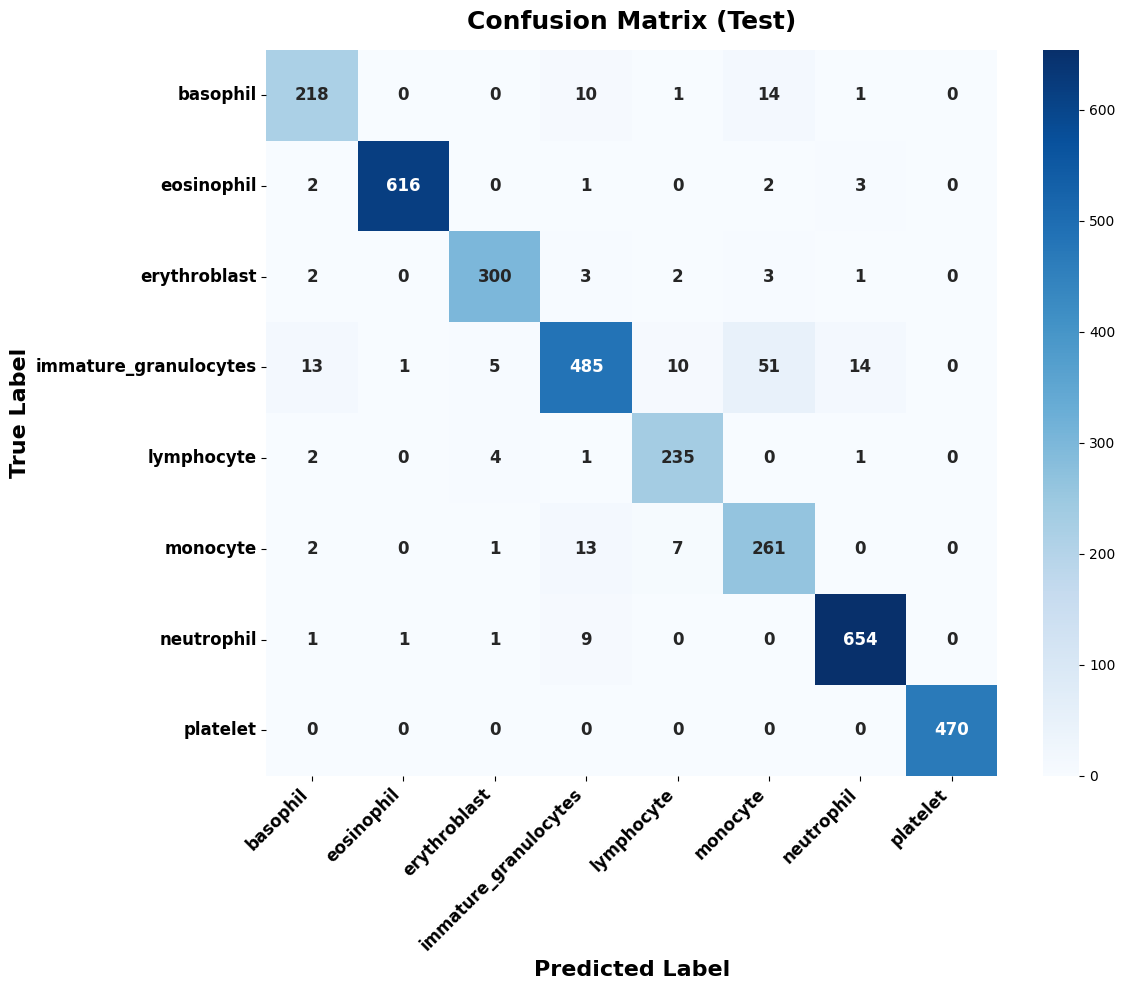
\includegraphics[width=0.6\linewidth]{confusion matrix1.png} 
    \caption{Confusion matrix on the BloodMNIST dataset. }
    \label{fig:breakhis_confusion}

\end{figure} 
\FloatBarrier
For the Raabin-WBC dataset, the model achieved 99.67\% training accuracy (loss: 0.0082) and 98.86\% validation accuracy (loss: 0.0212). Test results are reported in \autoref{tab:bach_metrics}, with the confusion matrix in \autoref{fig:bach_confusion}. 

Grad-CAM visualizations and t-SNE analysis are presented in \autoref{fig:gradcam_results} and \autoref{fig:tsne_results}, respectively.

\begin{table}[h!]
\centering
\caption{Results obtained on the Raabin-WBC dataset}
\vspace{3pt}
\label{tab:bach_metrics}
\resizebox{0.7\columnwidth}{!}{
\begin{tabular}{lcccc}
\hline
\textbf{Class} & \textbf{Precision} & \textbf{Recall} & \textbf{F1-score} & \textbf{Accuracy} \\
\hline
Basophil      & 0.9888 & 0.9897 & 0.9852 & 0.9869 \\
Eosinophil      & 0.9806 & 0.9801 & 0.9809 & 0.9807 \\
Lymphocyte      & 0.9412 & 0.9410 & 0.9409 & 0.9405 \\
Monocyte    & 0.9511 & 0.9515 & 0.9510 & 0.9530 \\
Neutrophil      & 0.9543 & 0.9541 & 0.9531 & 0.9533 \\ 
\hline
\textbf{Average}       & 0.9531 & 0.9542 & 0.9541 & 0.9550 \\
\hline
\end{tabular}
}
\end{table}


\begin{figure}[!ht]
    \centering
    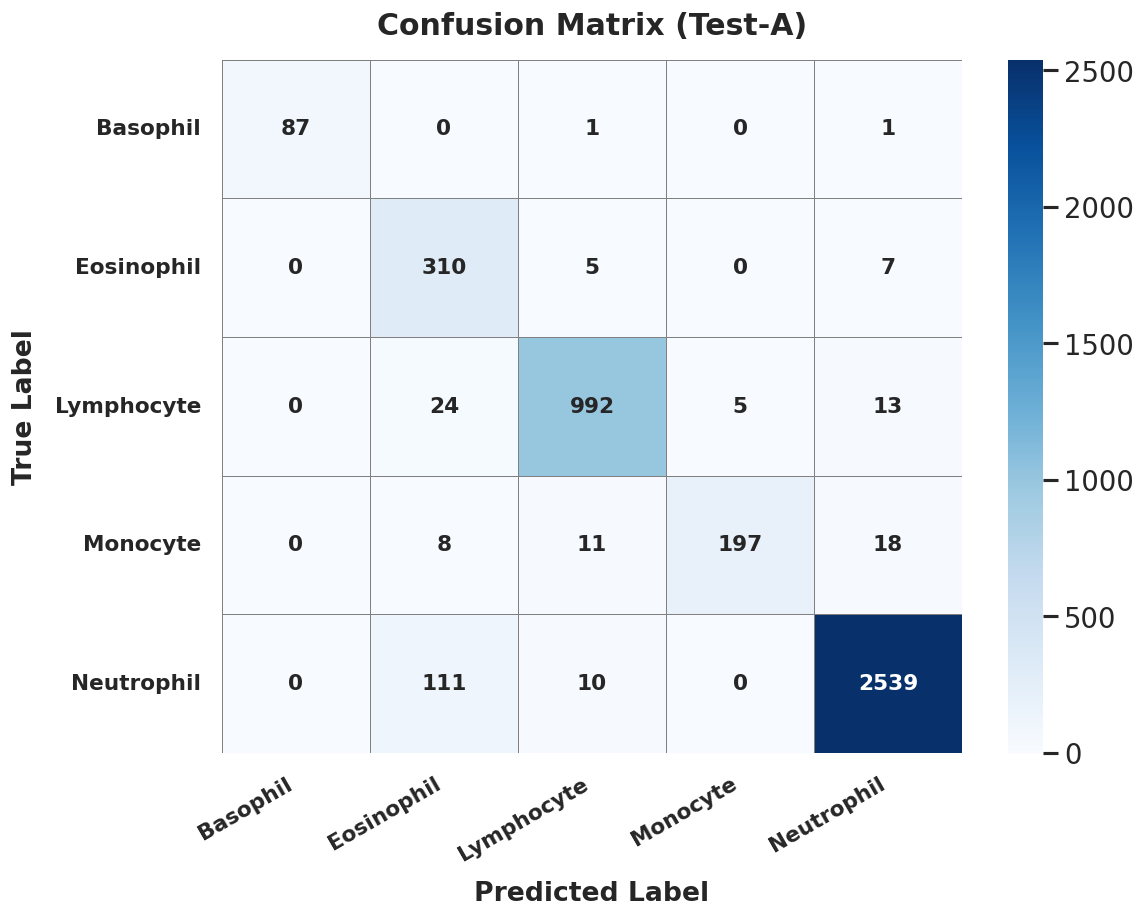
\includegraphics[width=0.5\linewidth]{confusion matrix3.png} 
    \caption{Confusion matrix of the Raabin-WBC dataset. }
    \label{fig:bach_confusion}
\end{figure} 

The confusion matrices \autoref{fig:breakhis_confusion}, \autoref{fig:bach_confusion} further support this interpretation that the improvement is not only due to increased parameterization, but also due to the interaction-aware fusion rule that modulates agreement and disagreement between branch-wise features. Most diagonal entries are strong, indicating high class-wise reliability, and the fused model reduces several off-diagonal confusions that remain visible in weaker baselines. In particular, classes with partially overlapping visual traits (e.g., granulocyte subtypes or morphologically close leukocyte categories) exhibit fewer mutual errors after fusion, implying better class boundary formation. At the same time, the residual off-diagonal pockets show that visually similar categories are still challenging under low-resolution or staining variability conditions. Therefore, the model is robust but not immune to fine-grained inter-class ambiguity, especially when diagnostic cues are subtle or partially occluded.


\FloatBarrier
\subsection{Visualization of Results}
Grad-CAM visualizations in \autoref{fig:gradcam_results} highlight the regions of interest used by the model for prediction. The attention maps consistently focus on salient cellular structures such as nuclei and cytoplasm, confirming that the model learns meaningful and clinically relevant features.

From a strengths perspective, the model offers: (i) strong cross-dataset performance as shown in \autoref{tab:breakhis_metrics}, \autoref{tab:bach_metrics}, (ii) clear ablation-backed contribution from each component \autoref{tab:ablation_bloodmnist}, (iii) improved explainability through Grad-CAM behavior \autoref{fig:gradcam_results}, and (iv) better feature geometry indicated by t-SNE structure \autoref{fig:tsne_results}. These attributes make the method promising for practical blood-cell analysis pipelines where both accuracy and interpretability matter. From a limitations perspective, several drawbacks remain. First, the approach introduces additional design complexity compared with simpler end-to-end backbones, including multiple branches and a non-trivial fusion rule. Second, although errors are reduced, confusion among morphologically similar classes persists, indicating limited robustness under severe class overlap. Third, t-SNE and saliency analyses are supportive but still post-hoc; they do not guarantee causal interpretability. Finally, performance has been validated on two datasets, and broader multi-center/domain-shift evaluation is still required for stronger clinical transfer claims.

These Grad-CAM visualizations in \autoref{fig:gradcam_results} provide additional qualitative evidence of improved decision behavior. Compared with isolated local/global branches, the fused branch tends to concentrate activation around diagnostically meaningful regions (nuclear contour, chromatin-rich interior, and relevant cytoplasmic texture) with less irrelevant background emphasis. This indicates that fusion not only changes final logits but also improves where the model attends. A practical implication is better interpretability for medical screening workflows: when attention maps align with expected cellular structures, clinicians can more readily trust the model’s outputs. However, some samples still show diffuse or slightly shifted activations, revealing that saliency stability is not yet uniform across all classes and image conditions.

Furthermore, the t-SNE projections in \autoref{fig:tsne_results} are consistent with the quantitative and Grad-CAM findings. Local and global embeddings individually show partial clustering with noticeable overlaps, while fused embeddings demonstrate tighter intra-class grouping and better inter-class separation. This geometric consolidation aligns with the proposed Choquet--Minkowski--Parseval mechanism, where agreement-aware weighting and distance-sensitive modulation help suppress conflicting branch evidence. Better manifold separation can explain the improved generalization seen in test metrics. 

Overall, the qualitative analyses reinforce the effectiveness of the proposed dual-branch fusion strategy. By jointly leveraging local texture sensitivity and global contextual awareness, the model achieves not only improved classification performance but also more structured and interpretable feature representations. The consistent alignment between attention maps, embedding geometry, and quantitative metrics suggests that the proposed Choquet–Minkowski–Parseval fusion mechanism enhances both discriminative capability and feature coherence. These results indicate that the model is not merely learning to classify, but is capturing clinically meaningful patterns in a stable and explainable manner, which is essential for reliable deployment in medical imaging applications.
\vspace{2.5cm}

\begin{figure*}[!htbp]
\centering

\setlength{\tabcolsep}{6pt}
\renewcommand{\arraystretch}{1.3}

\resizebox{0.75\linewidth}{!}{%   % reduced from 0.9 → 0.75
\begin{tabular}{c c c}

\textbf{Local} & \textbf{Global} & \textbf{Fusion} \\

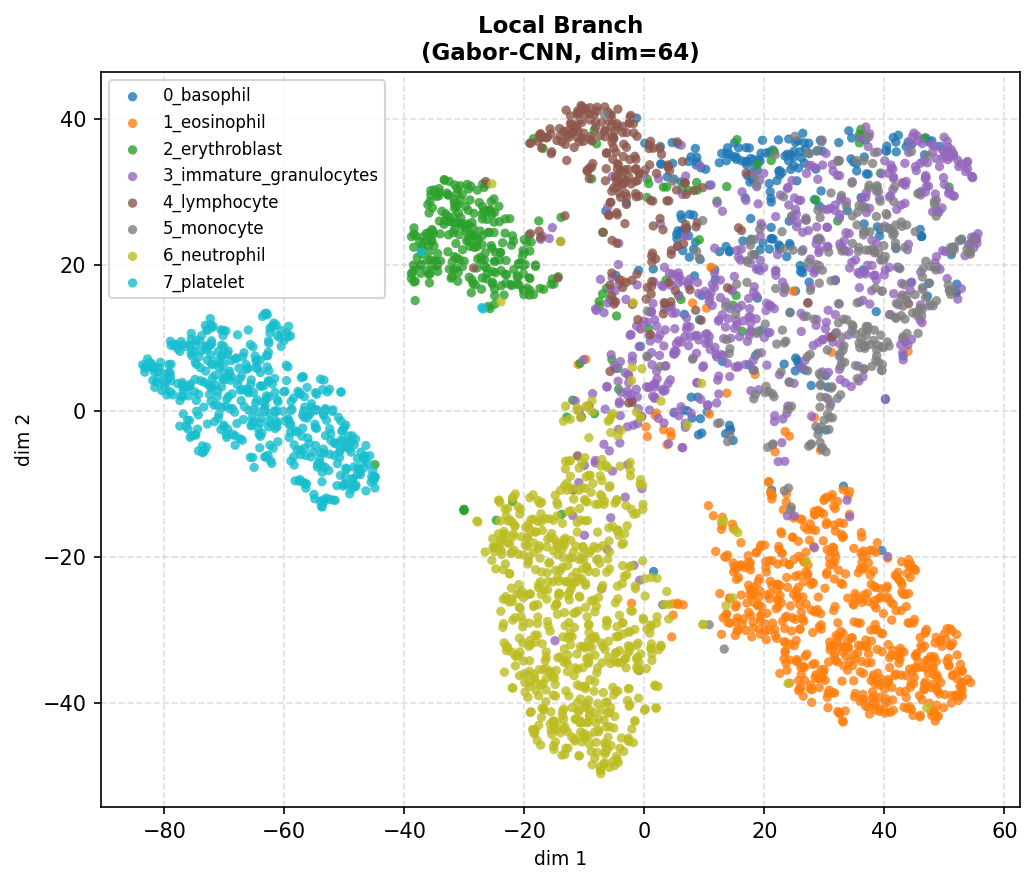
\includegraphics[width=0.55\linewidth]{tsne_local_branch (1).png} &
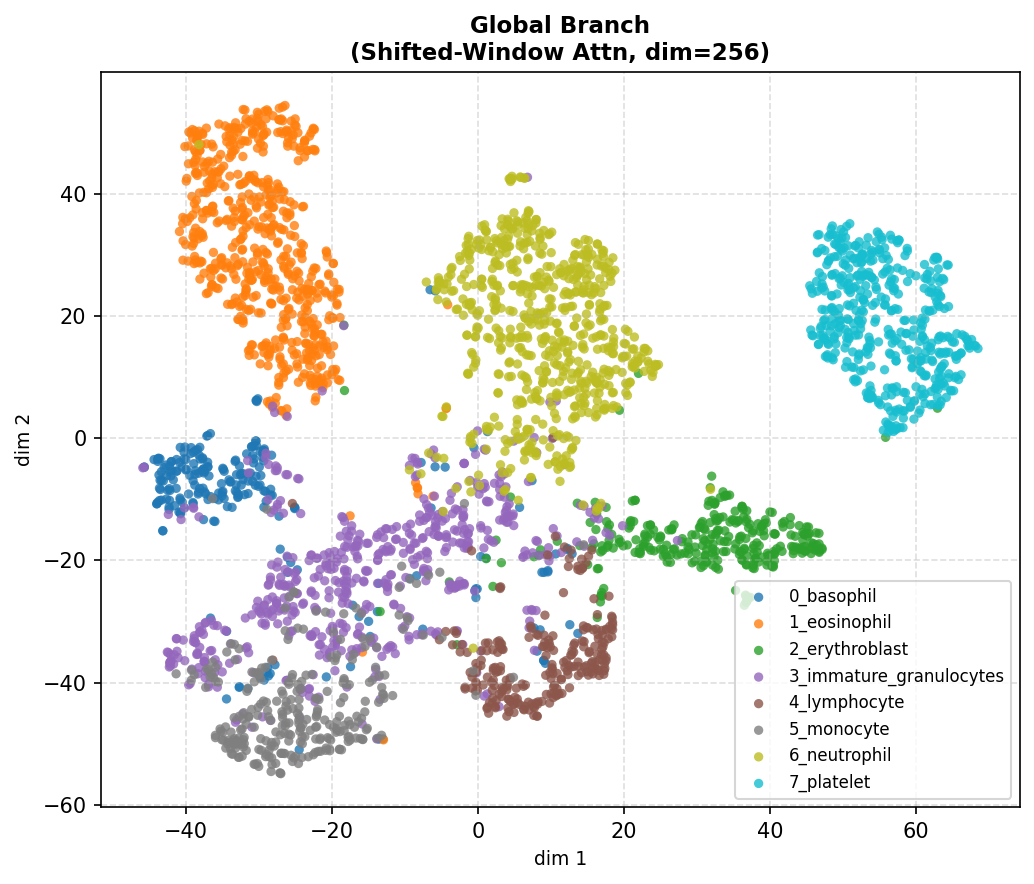
\includegraphics[width=0.55\linewidth]{tsne_global_branch (1).png} &
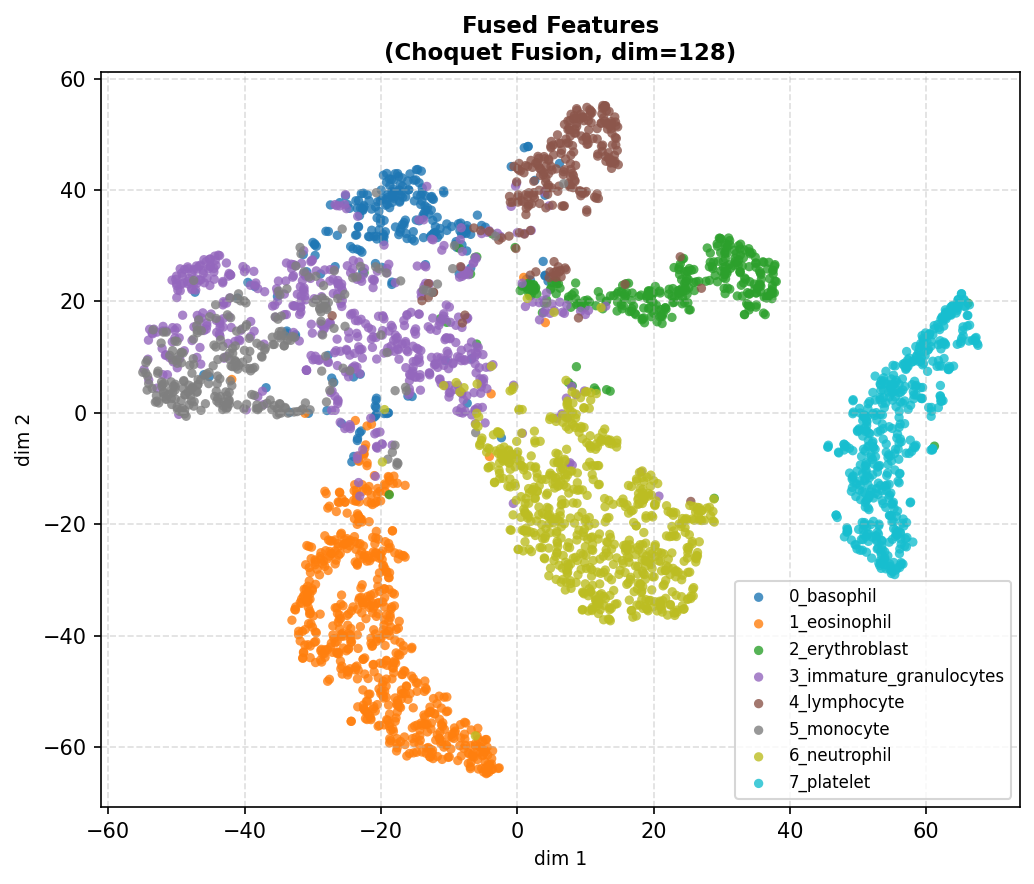
\includegraphics[width=0.55\linewidth]{tsne_fused (1).png} \\

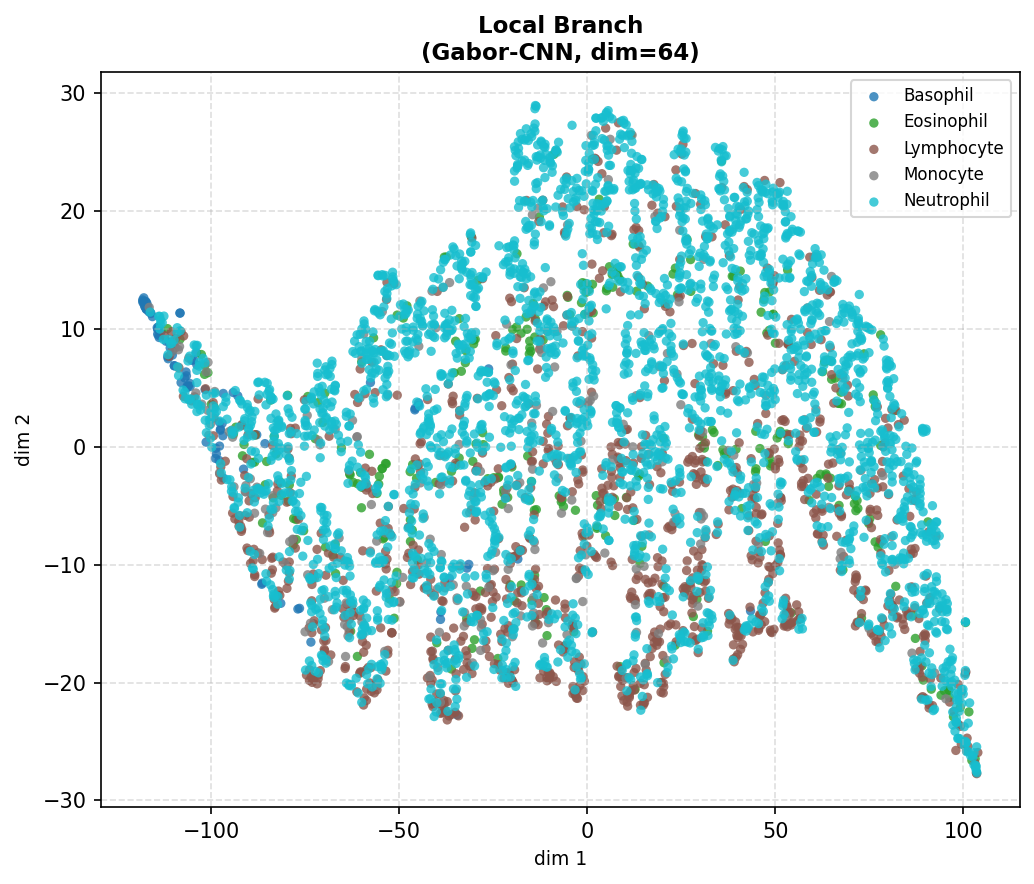
\includegraphics[width=0.55\linewidth]{tsne_local_branch.png} &
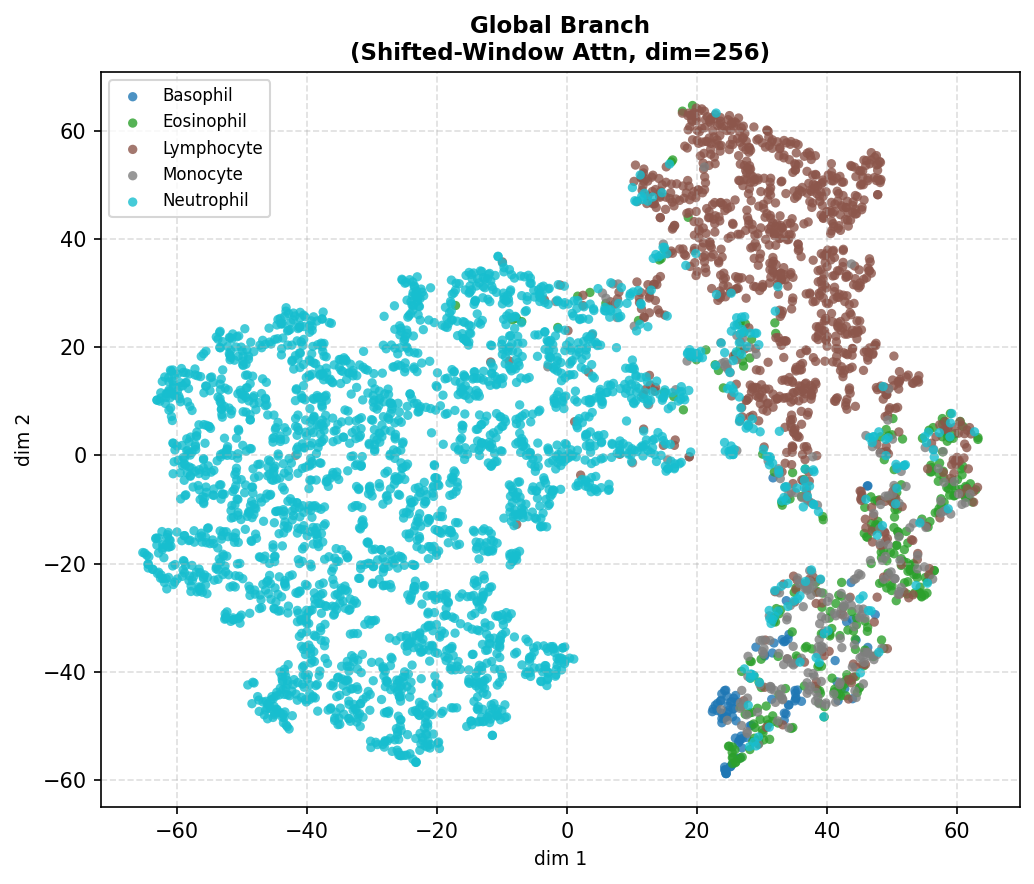
\includegraphics[width=0.55\linewidth]{tsne_global_branch.png} &
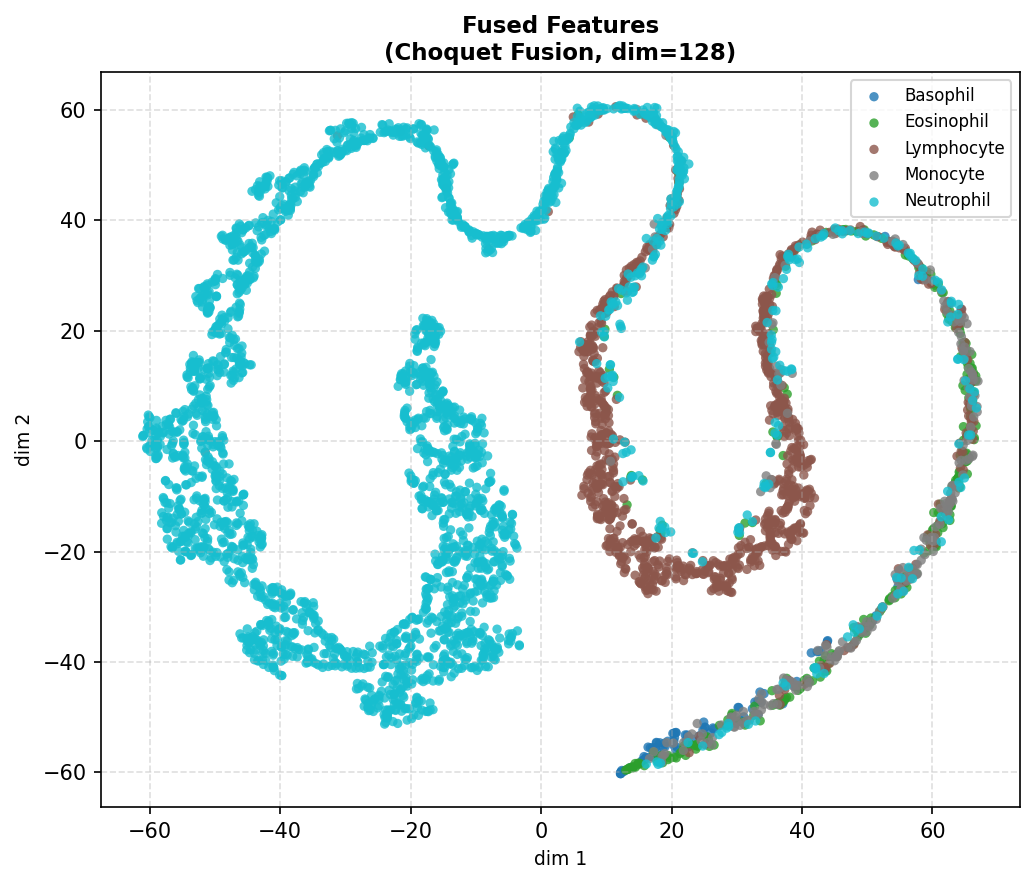
\includegraphics[width=0.55\linewidth]{tsne_fused.png}

\end{tabular}
}

\caption{t-SNE visualization of feature representations for BloodMNIST (top) and Raabin-WBC (bottom) datasets.}
\label{fig:tsne_results}

\end{figure*}

\begin{figure*}[!h]
\centering

% -------- Row 1 --------
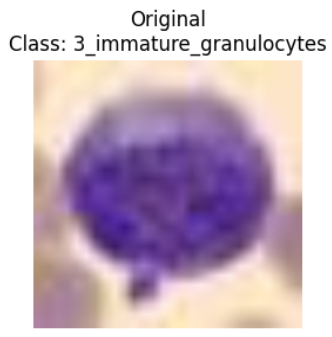
\includegraphics[width=0.20\linewidth,height=3.2cm]{gc1_granulo.png}
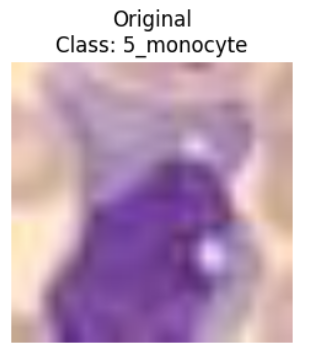
\includegraphics[width=0.20\linewidth,height=3.2cm]{gc1_monocyte.png}
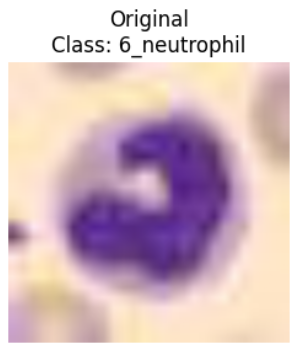
\includegraphics[width=0.20\linewidth,height=3.2cm]{gc1_neutrophil.png}
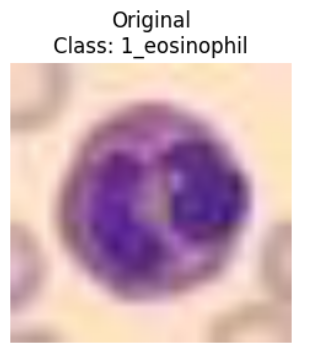
\includegraphics[width=0.20\linewidth,height=3.2cm]{gradcam1_eosinophil.png}

\vspace{0.15cm}

% -------- Row 2 --------
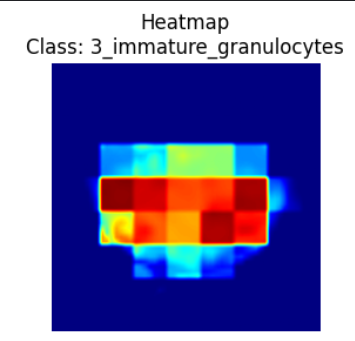
\includegraphics[width=0.20\linewidth,height=3.2cm]{gc1_granulo2.png}
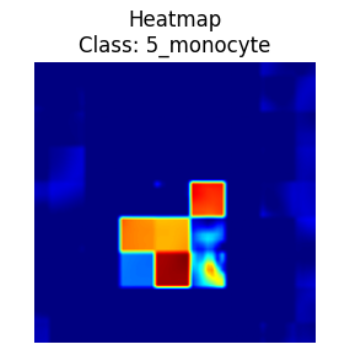
\includegraphics[width=0.20\linewidth,height=3.2cm]{gc1_monocyte2.png}
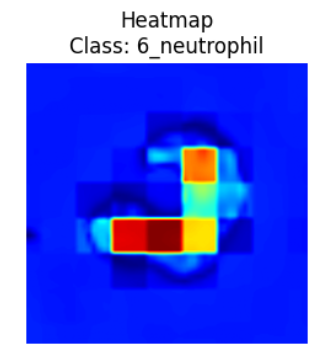
\includegraphics[width=0.20\linewidth,height=3.2cm]{gc1_neutrophil2.png}
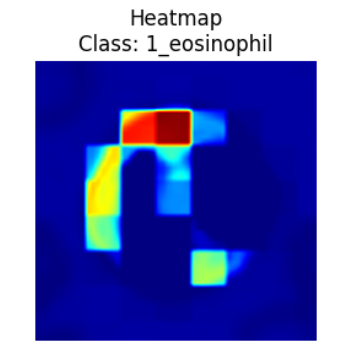
\includegraphics[width=0.20\linewidth,height=3.2cm]{gradcam1_eosinophil2.png}

\vspace{0.15cm}

% -------- Row 3 --------
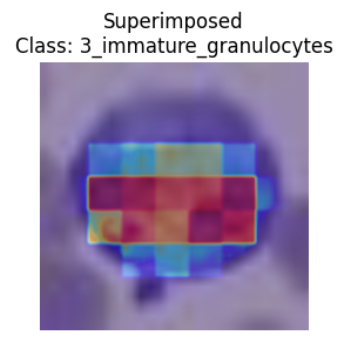
\includegraphics[width=0.20\linewidth,height=3.2cm]{gc1_granulo3.png}
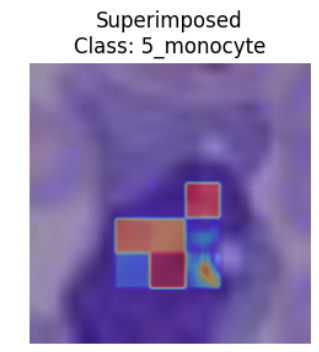
\includegraphics[width=0.20\linewidth,height=3.2cm]{gc1_monocyte3.png}
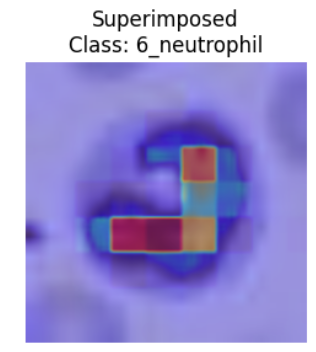
\includegraphics[width=0.20\linewidth,height=3.2cm]{gc1_neutrophil3.png}
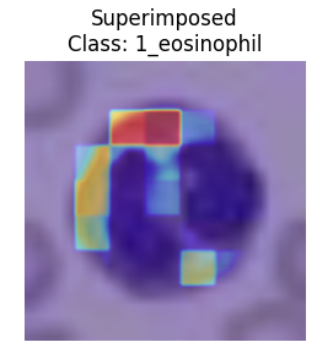
\includegraphics[width=0.20\linewidth,height=3.2cm]{gradcam1_eosinophil3.png}

\caption{Grad-CAM visualization: first row shows original images, second row shows heatmaps, and third row shows superimposed results for different blood cell classes.}
\label{fig:gradcam_results}

\end{figure*}


\FloatBarrier
\subsection{Comparative Results}
We present a comparative evaluation of the proposed method against
recent approaches on the BloodMNIST and Raabin-WBC
datasets in \autoref{tab:comparison} containing detals of authors, their models and detailed metrics inc;uding Accuracy (Acc), Precision (Prec), Recall (Rec), F1 Scores.

Overall, the findings from \autoref{tab:comparison} suggest that the proposed fusion strategy is a meaningful step beyond standard concatenation/averaging done in the previous attempts and provides a better balance between discriminative power and interpretability. 
%  

% The comparative results presented in \autoref{tab:comparison} demonstrate that the proposed dual-branch fuzzy fusion model consistently achieves competitive or superior performance across both datasets. 

\begin{table}[!t]
\centering
\caption{Performance comparison on BloodMNIST and Raabin-WBC datasets}
\label{tab:comparison}
\setlength{\tabcolsep}{2pt}
\renewcommand{\arraystretch}{1.25}
\resizebox{\columnwidth}{!}{
\begin{tabular}{|p{3.5cm}|p{4.1cm}|p{1.5cm}|p{1.5cm}|p{1.5cm}|p{1.5cm}|}
\hline
\multicolumn{6}{|c|}{\textbf{Dataset: BloodMNIST}} \\ \hline
\textbf{Author} & \textbf{Model} & \textbf{Acc} & \textbf{Prec} & \textbf{Rec} & \textbf{F1} \\ \hline

Shobiry et al. (2025)~\cite{b17} & EfficientNetV2 + SVM & 0.77 & 0.75 & 0.74 & 0.74 \\ \hline

Sengupta et al. (2025)~\cite{b39} & GCN  + Fuzzy & 0.88 & - & 0.86 & 0.86 \\ \hline

Radhi et al. (2024)~\cite{b16} & Quantum-EfficientNet & 0.96 & 0.95 & 0.96 & 0.95 \\ \hline


Patel et al. (2025)~\cite{b18} & Swin + CNN & 0.95 & 0.94 & 0.95 & 0.95 \\ \hline

Zhao et al. (2026)~\cite{b38} & FANL & 0.96 & 0.96 & 0.96 & 0.96 \\ \hline

O. Bilal et al. (2025)~\cite{b45} & Ensemble of 3 CNNS  & 0.95 & - & - & -  \\ \hline

Manzari et al.(2023)~\cite{b46} & MedViT-L & 0.95 & - & - & -  \\ \hline
\textbf{Proposed} & Fuzzy fusion model & \textbf{0.97} & \textbf{0.96} & \textbf{0.98} & \textbf{0.97} \\ \hline

\multicolumn{6}{|c|}{\textbf{Dataset: Raabin-WBC}} \\ \hline

% Gao et al. ~\cite{b22} & MobileNetV2 & 0.93 & 0.93 & 0.94 & 0.94 \\ \hline

% Toptaş et al. ~\cite{b20} & CNN Ensemble + SVM & 0.97 & 0.97 & 0.93 & 0.94 \\ \hline

% Zou et al. ~\cite{b19} & ICAFF-MobileNetV2 & 0.90 & 0.90 & 0.90 & 0.90 \\ \hline

% Baydilli et al. ~\cite{b21} & Capsule Network(Raabin-WBCaps) & 0.93 & 0.95 & 0.94 & 0.95 \\ \hline
% HMS-CycleGAN
% YOLOv8n-cls

Jiang et al. (2022)~\cite{b40} & DRFA-Net & 0.95 & 0.90 & 0.93 & 91.89 \\ \hline
Dhibar et al. (2025)~\cite{b41} & DCENWCNet & 0.93 & 0.85 & 0.94 & 0.88 \\ \hline
Tavakoli et al. (2021)~\cite{b42} & CNN + segmentation & 0.94 & - & - & - \\ \hline
Posada et al. (2022)~\cite{b43} & XceptionNet + SVM & 0.94 & 0.89 & 0.95 & 0.91 \\ \hline
Tavakoli et al. (2021)~\cite{b44} & CNN + segmentation + SVM & 0.94 & 0.89 & 0.92 & 0.91 \\ \hline


\textbf{Proposed} & Fuzzy fusion model & \textbf{0.95} & \textbf{0.96} & \textbf{0.95} & \textbf{0.95} \\ \hline

\end{tabular}
}
\end{table}

\FloatBarrier
\subsection{Ablation Studies}
To qualitatively evaluate the model performance, we analyze confusion patterns, class-discriminative attention, and feature space separability. Additionally, we compare the model complexity in terms of parameter count against standard pretrained architectures to highlight its lightweight nature.


\FloatBarrier
On the BloodMNIST dataset, the proposed method attains an accuracy of 0.98, outperforming several strong baselines including Swin + CNN and Quantum-EfficientNet variants. Notably, while existing methods achieve high performance through either advanced architectures or hybrid quantum-classical designs, the proposed approach achieves comparable or better results using a principled feature fusion strategy rather than relying solely on backbone complexity. This indicates that effective integration of complementary feature representations can be as impactful as increasing model depth or architectural sophistication.We compare the parameter count of the proposed model with standard pretrained architectures, as shown in Table~\ref{tab:param_comparison} to illustrate that our model is more lightweight than commonly used networks.

\begin{table}[!h]
\centering
\caption{Comparison of parameter count with standard pretrained models}
\vspace{3pt}
\label{tab:param_comparison}
\resizebox{0.7\columnwidth}{!}{
\small
\begin{tabular}{|l|c|c|}
\hline
\textbf{Model} & \textbf{Parameters (M)} & \textbf{Relative Size} \\ \hline

Proposed Model & 0.5 & 1$\times$ \\ \hline
MobileNetV2 & 3.4 & 6.8$\times$ \\ \hline
EfficientNet-B0 & 5.3 & 10$\times$ \\ \hline
ResNet-50 & $\sim$25.6 & 50$\times$ \\ \hline
Xception & $\sim$22.9 & 45$\times$ \\ \hline
VGG-16 & $\sim$138 & 275$\times$ \\ \hline

\end{tabular}
}
\end{table}


\begin{table}[!h]
\centering
\caption{Performance of different model variants on the BloodMNIST dataset}
\vspace{3pt}
\label{tab:ablation_bloodmnist}
\resizebox{0.7\columnwidth}{!}{
\small
\begin{tabular}{|l|c|c|}
\hline
\textbf{Model Variant} & \textbf{Train Acc (\%)} & \textbf{Test Acc (\%)} \\ \hline

CNN with Gabor(local) & 91.85 & 89.01 \\ \hline
CNN with SWMHSA(Global) & 91.65 & 89.72 \\ \hline
Simple concatenation                  & 95.69 & 92.73 \\ \hline
Weighted average                  & 95.28 & 94.77 \\ \hline
Fused by only Minkowski distance           & 94.87 & 92.53 \\ \hline
Fused by only Parseval identity  & 94.36 & 92.88 \\ \hline
Proposed fusion  & \textbf{98.33} & \textbf{97.37} \\ \hline

\end{tabular}
}
\end{table}

On the Raabin-WBC dataset, the proposed model achieves an accuracy of 0.95 with balanced precision, recall, and F1-score, demonstrating stable generalization across all classes. Although certain ensemble-based methods report slightly higher accuracy, they often rely on multiple models or heavier pipelines. In contrast, the proposed approach maintains a favorable trade-off between performance and architectural simplicity while still delivering competitive results.

\begin{table}[!h]
\centering
\caption{Performance of different model variants on the Raabin-WBC dataset}
\vspace{3pt}
\label{tab:ablation_Raabin-WBC}
\resizebox{0.7\columnwidth}{!}{
\small
\begin{tabular}{|l|c|c|}
\hline
\textbf{Model Variant} & \textbf{Train Acc (\%)} & \textbf{Test Acc (\%)} \\ \hline

CNN with Gabor(local) & 91.33 & 90.25 \\ \hline
CNN with SWMHSA(Global) & 91.57 & 90.92 \\ \hline
Simple concatenation                  & 95.14 & 93.78 \\ \hline
Weighted average                  & 95.29 & 93.75 \\ \hline
Fused by only Minkowski distance           & 90.64 & 88.70 \\ \hline
Fused by only Parseval identity  & 94.35 & 93.06 \\ \hline
Proposed fusion  & \textbf{97.29} & \textbf{95.37} \\ \hline

\end{tabular}
}
\end{table}

Overall, the results suggest that the primary strength of the proposed method lies in its ability to effectively combine local texture-sensitive features and global contextual representations. The Choquet-inspired fuzzy fusion mechanism enables interaction-aware aggregation, allowing the model to reinforce complementary information while suppressing conflicting evidence, leading to more consistent performance.


\FloatBarrier
 \section{Conclusion}
In this work, we proposed MPC-net a novel lightweight dual-branch deep learning framework for blood cell classification that effectively integrates complementary feature representations. The architecture combines a Gabor-based CNN branch for capturing fine-grained local texture and orientation information with a shifted window attention-based CNN branch for modeling global contextual dependencies. To unify these heterogeneous features, we introduced a Choquet integral-inspired fuzzy fusion mechanism enhanced with Minkowski distance-based geometric modulation and Parseval-driven energy alignment, enabling adaptive, interaction-aware feature aggregation.

Experimental results demonstrate that this dual-branch design consistently outperforms single-branch and conventional fusion baselines. While the Gabor-CNN branch captures orientation-sensitive micro-textures and the attention branch encodes broader contextual structure, their combination through the proposed fusion strategy yields a significant performance gain on both BloodMNIST and Raabin-WBC. Ablation studies confirm that this improvement stems not merely from increased architectural complexity, but from principled modeling of feature interactions, effectively reinforcing agreement and suppressing conflicting representations.

Further validation through quantitative metrics and qualitative analyses, including Grad-CAM and t-SNE, indicates improved interpretability and feature-space separability. These results suggest that the proposed fusion mechanism enhances both discriminative capability and representation coherence.

Despite these strengths, certain limitations remain. The model introduces additional architectural and computational complexity, and some misclassifications persist among morphologically similar classes, particularly under low-resolution or ambiguous conditions. Moreover, evaluation on only two datasets limits insights into broader real-world generalization.

Future work will focus on extending the fusion framework with more advanced or learnable aggregation strategies, improving robustness through domain adaptation and stain normalization, and validating performance on larger, multi-center datasets. Incorporating uncertainty estimation and model optimization for efficiency will further support practical clinical deployment.

\textbf{Acknowledgements.} The authors acknowledge the CMATER Research Laboratory, Department of Computer Science and Engineering (CSE), Jadavpur University, Kolkata, India. This research work was supported by the ongoing FIST program of the Department of CSE, Jadavpur University, titled ‘FIST Engineering Sciences Level B/C/D Project’. The program is funded by the Department of Science and Technology, Government of India, under reference number SR/FST/ET-I/2022/1059(C).


\begin{thebibliography}{00}
\bibitem{b37}
Alzubaidi, Laith, et al. "Review of deep learning: concepts, CNN architectures, challenges, applications, 
future directions." Journal of big Data 8.1 (2021): 53.

\bibitem{b33}
Mehrotra, Rajiv, Kameswara Rao Namuduri, and Nagarajan Ranganathan. "Gabor filter-based edge detection." Pattern recognition 25.12 (1992): 1479-1494.

\bibitem{b34}
Liu, Ze, et al. "Swin transformer: Hierarchical vision transformer using shifted windows." Proceedings of the IEEE/CVF international conference on computer vision. 2021.

\bibitem{b35}
Grabisch, Michel, and Marc Roubens. "Application of the Choquet integral in multicriteria decision making." Fuzzy Measures and Integrals-Theory and Applications (2000): 348-374.

\bibitem{b36}
Xu, Hang, et al. "An evolutionary algorithm based on Minkowski distance for many-objective optimization." IEEE transactions on cybernetics 49.11 (2018): 3968-3979.

\bibitem{b43}
Rivas-Posada, Eduardo, et al. "Classification of leukocytes using meta-learning and color constancy methods." Jurnal Ilmiah Teknik Elektro Komputer dan Informatika (JITEKI) 8.4 (2022): 486-499.

\bibitem{b17}
A. K. F. Shobiry and R. Puspitasari,
``Hybrid Feature Benchmark for Blood Cell Classification Using ResNet50 and EfficientNetV2 Features with SVM and ANN Classifiers via Unsupervised Segmentation,''
International Journal of Artificial Intelligence and Machine Intelligence (IJAIMI),
Vol. 3, No. 2, 2024, doi: 10.56705/ijaimi.v3i2.364.

\bibitem{b41}
Dhibar, Sibasish. "DCENWCNet: A deep CNN ensemble network for white blood cell classification with LIME-based explainability." arXiv preprint arXiv:2502.05459 (2025).

\bibitem{b38}
Zhao, Zheng, Doo Heon Song, and Kwang Baek Kim. "Fuzzy Attention Convolutional Neural Networks: A Novel Approach Combining Intuitionistic Fuzzy Sets and Deep Learning." Computers, Materials,  Continua 87.2 (2026).

\bibitem{b45}
Bilal O, Asif S, Zhao M, Khan SUR et, Li Y (2025) An amalgamation of deep neural networks optimized with salp swarm algorithm for cervical cancer detection. 123:110106 Computers and Electrical Engineering

\bibitem{b46}
Manzari O, Ahmadabadi H, Kashiani H, Shokouhi S, Ayatollahi A (2023) Medvit: a robust vision transformer for generalized medical image classification. Comput Biol Med 157:106791

\bibitem{b39}
Sengupta, Prajit, and Islem Rekik. "FireGNN: Neuro-Symbolic Graph Neural Networks with Trainable Fuzzy Rules for Interpretable Medical Image Classification." arXiv preprint arXiv:2509.10510 (2025).

\bibitem{b16}
E. A. Radhi, M. A. Mohammed, F. Eid and I. de la Torre Díez,
``Efficient Blood Cell Classification Using a Hybrid Variational Quantum Circuit–EfficientNet Model on BloodMNIST,''
Journal of Artificial Intelligence and Medical Applications (JAIMA),
Vol. 1, No. 1, 2023, doi: 10.65511/jaima.v1i1.734.

\bibitem{b42}
Tavakoli, Sajad, Ali Ghaffari, and Zahra Mousavi Kouzehkanan. "Generalizability in white blood cells’ classification problem." BioRxiv (2021): 2021-05.

\bibitem{b44}
Tavakoli, Sajad, et al. "New segmentation and feature extraction algorithm for classification of white blood cells in peripheral smear images." Scientific Reports 11.1 (2021): 19428.

\bibitem{b1}
D. Gabor,
``Theory of Communication,''
Journal of the Institution of Electrical Engineers (JIEE), Vol. 93, Part III, pp. 429--457, 1946.

\bibitem{b2}
A. K. Jain and F. Farrokhnia,
``Unsupervised Texture Segmentation Using Gabor Filters,''
IEEE Transactions on Pattern Analysis and Machine Intelligence (PAMI),
Vol. 13, No. 11, pp. 1167--1186, 1991.

\bibitem{b3}
T. S. Lee,
``Image Representation Using 2D Gabor Wavelets,''
IEEE Transactions on Pattern Analysis and Machine Intelligence (PAMI),
Vol. 18, No. 10, pp. 959--971, 1996.

\bibitem{b4}
A. Vaswani, N. Shazeer, N. Parmar, J. Uszkoreit, L. Jones, A. N. Gomez, 
L. Kaiser and I. Polosukhin,
``Attention Is All You Need,''
Advances in Neural Information Processing Systems (NeurIPS),
pp. 5998--6008, 2017.

\bibitem{b5}
Z. Liu, Y. Lin, Y. Cao, H. Hu, Y. Wei, Z. Zhang, S. Lin and B. Guo,
``Swin Transformer: Hierarchical Vision Transformer Using Shifted Windows,''
Proceedings of the IEEE/CVF International Conference on Computer Vision (ICCV),
pp. 10012--10022, 2021.

\bibitem{b6}
G. Choquet,
``Theory of Capacities,''
Annales de l’Institut Fourier,
Vol. 5, pp. 131--295, 1953--1954.

\bibitem{b32}
H.~Bustince, R.~Mesiar, J.~Fernandez, M.~Galar, D.~Paternain, A.~Altalhi, G.~P. Dimuro, B.~Bedregal, and Z.~Takáč,
``d-Choquet integrals: Choquet integrals based on dissimilarities,''
\emph{Fuzzy Sets and Systems}, vol.~414, pp.~1--27, 2021.

\bibitem{b7}
M. Grabisch, T. Murofushi and M. Sugeno,
``Fuzzy Measures and Integrals: Theory and Applications,''
Studies in Fuzziness and Soft Computing, Springer,
Vol. 40, 2000.

\bibitem{b8}
M. Grabisch, J.-L. Marichal, R. Mesiar and E. Pap,
``Aggregation Functions,''
Encyclopedia of Mathematics and its Applications, Cambridge University Press,
Vol. 127, 2009.

\bibitem{b9} 
H. Minkowski,
``Beiträge zur Theorie der konvexen Körper,''
Nachrichten von der Gesellschaft der Wissenschaften zu Göttingen, 
Mathematisch-Physikalische Klasse, pp. 198--219, 1896.

\bibitem{b10}
X. Zhu and D. L. Smith,
``Comparison of Distance Measures in Spatial Analytical Modeling,''
Proceedings of the International Conference on Geographic Information Science (GIScience),
pp. 1--12, 2004.

\bibitem{b15}
A. O. Boudraa, J. C. Cexus and Z. Saidi,
``An Energy-Based Similarity Measure for Time Series,''
IEEE International Conference on Acoustics, Speech, and Signal Processing (ICASSP),
pp. 1973--1976, 2008.
2023.

\bibitem{b14}
T. Tanimoto,
``An Elementary Mathematical Theory of Classification and Prediction,''
IBM Internal Report, 1958.

\bibitem{b18}
T. Patel, H. El-Sayed, M. K. Sarker, D. Duong and B. D. Solomon,
``Training Swin Transformer-Based GAN for High-Resolution Blood Cell Imaging with Limited Data,''
Computational Science and Computational Intelligence (CSCI 2024),
Communications in Computer and Information Science (CCIS), Vol. 2511,
pp. 161--176, Springer, 2025.

\bibitem{b22}
W. Gao, L. Lan and X. Fan,
``DaNet: Domain-Adaptive White Blood Cell Classification Through Synthetic Augmentation and Cross-Domain Feature Alignment,''
Array,
2025, doi: 10.1016/j.array.2025.100416.

\bibitem{b20}
B. Toptaş, M. K. Öztürk and H. T. Kahraman,
``Classification of White Blood Cells Using CNN Ensemble and Support Vector Machine,''
Biomedical Signal Processing and Control,
Vol. 66, 2021.

\bibitem{b19}
Y. Zou, L. Wu, C. Zuo, L. Chen, B. Zhou and H. Zhang,
``White Blood Cell Classification Network Using MobileNetV2 with Multiscale Feature Extraction Module and Attention Mechanism,''
Biomedical Signal Processing and Control,
Vol. 91, 2024, doi: 10.1016/j.bspc.2024.106820.

\bibitem{b21}
Y. Y. Baydilli and Ü. Atila,
``Classification of White Blood Cells Using Capsule Networks,''
Computerized Medical Imaging and Graphics,
Vol. 80, 2020, doi: 10.1016/j.compmedimag.2020.101699.

\bibitem{b40}
Jiang, Lei, Chang Tang, and Hua Zhou. "White blood cell classification via a discriminative region detection assisted feature aggregation network." Biomedical optics express 13.10 (2022): 5246-5260.

\bibitem{b11}
M.-A. Parseval des Chênes,
``Über Fourierreihen,''
Mémoires présentés à l’Institut des Sciences, Lettres et Arts, 
pp. 638--648, 1799.

\bibitem{b12}
A.-L. Cauchy,
``Cours d’Analyse de l’École Royale Polytechnique,''
Imprimerie Royale, Paris, 1821.

\bibitem{b13}
H. A. Schwarz,
``Gesammelte mathematische Abhandlungen,''
Springer, Berlin, 1890.
\end{thebibliography}

\end{document}
